%---------------------------------------------------------------------------------
\chapter{Hybrid-Duplex UAV Communication in Rician Shadowed Fading Environments}
\label{chap:HBD_UCS_Rician_Shadowed}
%---------------------------------------------------------------------------------
\section{Introduction}

In Chapter \ref{chap:JD_HBD_UCS}, the performance of II-based, SIC-based, and JD-based HBD-UCSs operating in Rician fading environments was studied as a potential solution to address spectrum scarcity in UAV communications. Although Rician fading channels are commonly encountered in UAV communications, transmissions in practice are also impaired by the combined effect of fading and shadowing \cite{matolak2015unmannedAircraft,matolak2012air}, especially in urban environments \cite{al2014optimal}.\footnote{The work in this chapter has been published in \cite{ernest2019power}.}

To begin modeling a realistic UAV communication channel, it is first noted that channel measurement campaigns for UAV-to-ground links showed a \textcolor{black}{close match between the measurement data and the Rician fading model \cite{sun2017air_hilly}}. For UAV-to-UAV links, i.e., inter-UAV channels, measurement campaigns in \cite{goddemeier2015investigation} have also demonstrated the Rician fading channel as a suitable model for inter-UAV links. \textcolor{black}{The authors in \cite{yuan2018capacity} similarly employ} the Rician fading model for inter-UAV links to account for the availability of LOS links, scattering, and reflection from the environment. Nonetheless, despite several recent works on UAV channel modeling, e.g., \cite{zeng20173d,jin2017three,jiang2019three,jiang2018three}, channel models that jointly account for fading and shadowing have not been investigated extensively. In particular, the Rician fading model may not be accurate in a suburban environment as it does not account for shadowing due to terrain or buildings \cite{matolak2015unmannedAircraft,matolak2012air,al2014optimal}. In the empirical data of \cite{sun2017air_hilly}, where the characterization of UAV communication channels in hilly terrain was studied, Rician shadowed fading, i.e., LOS blockage, was observed. However, due to the limited dynamic range of the transceiver used during the measurement campaign, the authors in \cite{sun2017air_hilly} omitted measurement data containing LOS shadowing.

In light of the above limitations, the Rician shadowed fading model presented in \cite{tan2018ricianShad} is a suitable choice for UAV channel modeling. Through the Rician shadowed fading model, Rician fading or Rayleigh fading UAV channels \cite{ernest2018hybrid} can be modeled as special cases. It is worth noting that the Rician shadowed fading model is one of several shadowed fading, i.e., composite fading, models available in the literature. \textcolor{black}{Such composite fading models combine shadowing, i.e., large-scale fading, with small-scale fading, e.g., $\kappa - \mu$ or Rician fading\footnote{Small-scale fading occurs when the received signal power undergoes variations due to LOS or NLOS components, multipath clustering with circularly symmetric or elliptical scattering, and power imbalance between the in-phase and quadrature signal components \cite{chun2017comprehensive}. Depending on the type of environment, different kinds of small-scale fading can occur. For instance, Rician fading is commonly encountered in UAV communications \cite{matolak2017air_suburban}, \cite{sun2017air_hilly}, which can be modeled using the non-centered Chi-squared distribution.}. Also, fluctuations caused by shadowing are modeled using Gaussian, lognormal, gamma, or inverse Gaussian distributions \cite{al2014optimal,chun2017comprehensive}}.\footnote{Shadowing occurs when a communication link is obstructed by buildings or terrain \cite{matolak2015unmannedAircraft, matolak2012air, al2014optimal, chun2017comprehensive}, causing the total received signal power to fluctuate randomly \cite{chun2017comprehensive}. The resultant fluctuations can be modeled using the Gaussian, lognormal, gamma, or inverse Gaussian distributions \cite{al2014optimal, chun2017comprehensive}.} For the Rician shadowed fading model, one can employ the $\kappa - \mu$ shadowed fading model, where the non-centered Chi-squared and Nakagami-$m$ distributions are assumed for the multipath and LOS components, respectively \cite{chun2017comprehensive,paris2014statistical,zhang2017high,li2017effective}. In particular, the non-centered Chi-squared distribution accounts for both the LOS and NLOS components encountered over the UAV channel, while the degree of LOS shadowing is modeled through the Nakagami-$m$ distribution. Thus, using the Rician shadowed fading model, the severity of LOS shadowing and the ratio of the LOS-to-NLOS components can be accurately captured through the Nakagami-$m$ shaping parameter and the Rician $K$ factor, respectively. Furthermore, in contrast to the $\kappa - \mu$ shadowed fading model which considers LOS and NLOS shadowing for more than one multipath cluster, only one multipath cluster with LOS shadowing is considered for the Rician shadowed fading model. On top of the Rician shadowed fading model, it was shown by Paris \cite{paris2014statistical} that the $\kappa - \mu$ shadowed fading model includes the one-sided Gaussian, Rayleigh, $\kappa - \mu$, and Rician fading models as special cases, obtainable through the substitution of appropriate shaping parameters. However, the relevant statistics from \cite{chun2017comprehensive} and \cite{paris2014statistical} are represented in the form of complicated functions, such as the confluent hypergeometric function \cite{gradshteyn2014table} and the Gauss hypergeometric function \cite{kumar2015approximate}, which may not yield tractable solutions. \textcolor{black}{Hence}, one can adopt the Rician shadowed fading model presented in \cite{tan2018ricianShad}. In particular, the work in \cite{tan2018ricianShad} presented power series expressions for statistics in the Rician shadowed fading model. While the closed-form expressions in  \cite{tan2018ricianShad} enables tractable mathematical analysis, the generality of the Rician shadowed fading model using the power series approach, i.e., to obtain the Rician fading model, remains an open research problem which will be investigated in this chapter.

Although UAV communications in the presence of shadowing has been studied in the literature, e.g., \cite{motlagh2016uav,al2017modeling,amorim2017radio}, these works have not considered Rician shadowed fading or Rician fading and are only valid for interference-free scenarios. For interference management strategies, the II approach has already been investigated from the outage probability perspective for aeronautical communications over Rician fading channels \cite{ernest2019outage,ernest2018performance}, and for UAV communications over Rician fading channels \cite{ernest2018hybrid} and Rician shadowed fading channels \cite{tan2018ricianShad}. In particular, the work in \cite{tan2018ricianShad} presented new power series expressions for statistics associated with the Rician shadowed fading model. Thereafter, closed-form outage probability expressions for the II detector involving SINRs of the form $\frac{Z_0}{1+Z_1}$, where $Z_0$ and $Z_1$ denote the desired and interfering signals, respectively, were derived for the Rician shadowed fading model through a power series approach. Thus, through the power series approach in \cite{tan2018ricianShad}, one can easily obtain closed-form outage probability expressions for the II detector over Rician shadowed fading channels. In contrast, one may have to resort to numerical methods to evaluate the outage probability of the II detector using the statistics presented in \cite[eq. (3)]{abdi2003new}, \cite[eq. (12)]{chun2017comprehensive}, and \cite[eq. (4)]{paris2014statistical}. For the JD strategy, closed-form outage probability expressions are only available for Rician fading channels, e.g., \cite{tan2018joint}. Therefore, the outage probability analysis of UAV communications for JD over Rician shadowed fading channels through closed-form expressions remains an open problem.

To this end, we extend the Rician shadowed fading model in \cite{tan2018ricianShad} to include the Rician fading model as a special case. It is worth mentioning that closed-form power series expressions for the Rician fading model are already available in \cite[Table I and Table II]{rached2017unified}. However, we present alternative power series representations for the Rician fading model using the Rician shadowed fading model in this chapter. \textcolor{black}{We} demonstrate that the Rician shadowed fading model in this chapter unifies Rician shadowed fading, Rician fading, and Rayleigh fading under the same power series-based model. Through the newly obtained closed-form expressions for the Rician shadowed fading model, we conduct an outage probability analysis of HBD UAV communications for multi-UAV networks in both Rician shadowed fading and Rician fading environments. Specifically, the outage probability analysis takes into consideration the effects of inter-UAV interference, SI, fading, and shadowing for the II and JD interference management approaches. Additionally, it is worth noting that this chapter is an extension of the work in \cite{tan2018ricianShad}, where the UAV-to-GS and the SI links are modeled as Rician fading channels. \textcolor{black}{The} current chapter models the UAV channels and SI channel using the Rician shadowed fading model. As such, the system model and the subsequent analysis in \cite{tan2018ricianShad} can be obtained in this chapter as specific cases, thus illustrating the generality of the employed Rician shadowed fading model in this chapter. 

%Thus, the main contributions of this paper are summarized below.
%
%% Major contributions
%\subsection{Main Contributions}
%\begin{itemize}
%\item The present paper proposes a novel approach towards obtaining alternative power series representations of the probability density function (PDF), cumulative distribution function (CDF), and fractional moment for both the Rician fading and the Rician shadowed fading models.
%\item From the derived equations, closed-form outage probability expressions for the II and joint detectors using alternative power series expressions for the Rician shadowed fading and Rician fading models are obtained. To the best of our knowledge, the closed-form outage probability expressions and analysis are unavailable in the literature.
%\item Although counter-intuitive, it is shown that the impact of shadowing on the SI link at the FD-enabled GS is negligible. We also show that severe shadowing on the desired link with strong LOS component, as compared to weak LOS component, causes reduction in reliability even when SI mitigation measures are implemented.
%\item At UAV-2, the effect of severe shadowing on the desired link with strong LOS components is shown to be less severe for the joint detector than for the II detector.
%\end{itemize}
%
%% Organization of the paper
%The remainder of this paper is organized as follows. The system model is introduced in Section \ref{sec_sys_model}, with alternative expressions for both Rician fading and Rician shadowed fading models presented in Section \ref{sec_rician_shad}. Outage probability expressions are presented in Section \ref{sec_outage}, with numerical results discussed in Section \ref{sec_num_res} before the conclusion of the paper in Section \ref{sec_conclusion}.

%%%%%%%%%%%%%%%%%%%%%%%%%%%%%%%%%%%%%%%%%%%%%%%%%%%%%%%%%%%%%%%%%%%%%%%%%%%%%%%%%%%%%%%%%%%%%%%%%%%%%%%%%%%%%%%%%%%%%%%%%%%%%%%%%%%%%%%%%
% Section 2 : System Model
\section{System Model} \label{HBD_UCS_Rician_Shadowed_sec_sys_model}
%\vspace{-1cm}
\begin{figure} [tpb]
\centering
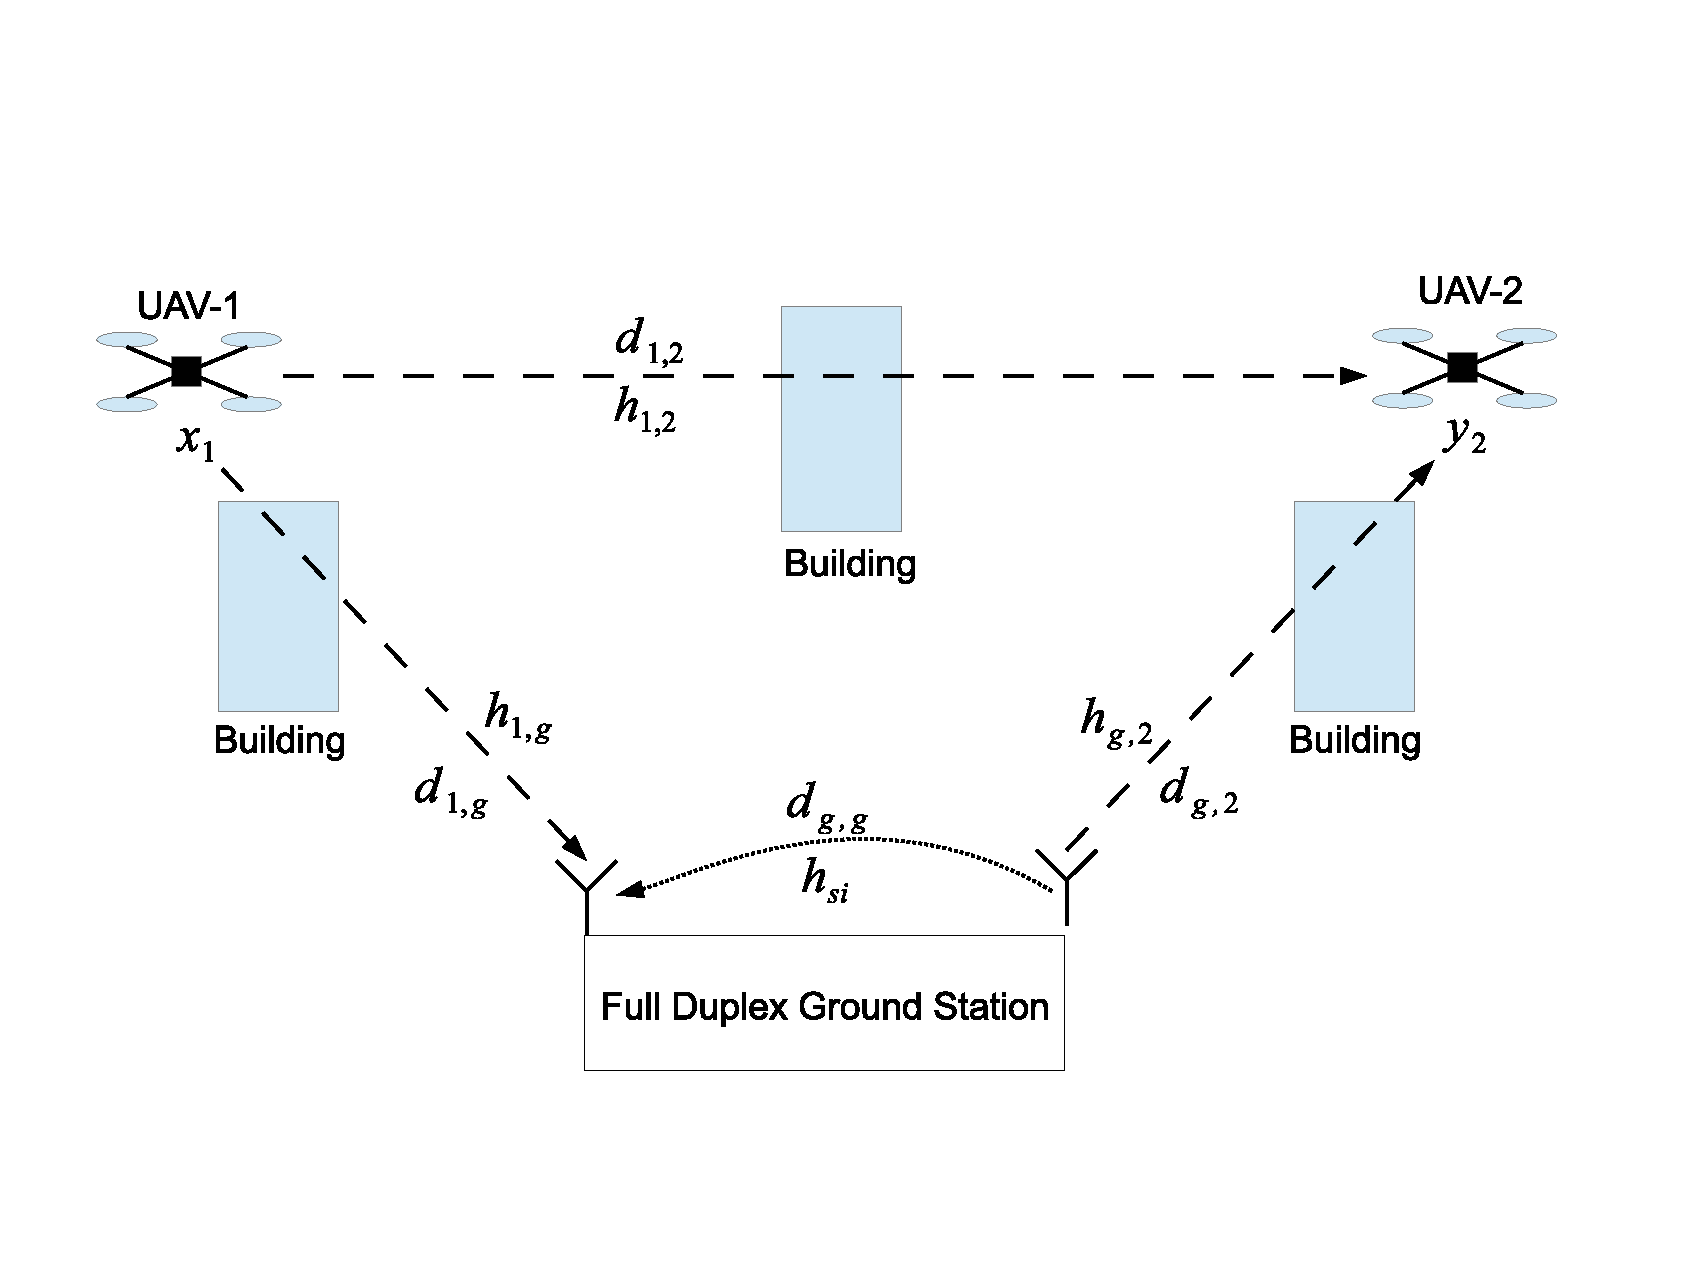
\includegraphics [width=0.5\columnwidth]{chap5_fig/block_diagram.eps}
\vspace{-1cm}
\caption{Unmanned Aerial Vehicle 1 (UAV-1) and Unmanned Aerial Vehicle 2 (UAV-2) operating in HD mode while communicating with the FD GS over Rician shadowed fading channels.}
%\vspace{-1cm}
\label{fig:HBD_UCS_Rician_Shadowed_block_diagram}
%\vspace{-0.3in}
\end{figure}

The multi-UAV HBD-UCS operating in a suburban environment is shown in Fig. \ref{fig:HBD_UCS_Rician_Shadowed_block_diagram}. In particular, it is assumed that the HD UAV-1 is simultaneously transmitting data to the FD-enabled GS while the HD UAV-2 is receiving control information on the same channel (Fig. \ref{fig:HBD_UCS_Rician_Shadowed_block_diagram}). Such an arrangement enables the HBD-UCS to utilize spectrum efficiently, which is a challenge in UAV communications \cite{matolak2017air_suburban}. Another major issue in multi-UAV networks is the interference present in the HBD-UCS \cite{motlagh2016low}. In Fig. \ref{fig:HBD_UCS_Rician_Shadowed_block_diagram}, signals from Unmanned Aerial Vehicle 1 (UAV-1) are transmitted to both GS and Unmanned Aerial Vehicle 2 (UAV-2) as the SOI and interference, respectively. Simultaneously at the FD-enabled GS, signals are transmitted to UAV-2. Consequently, inter-UAV interference and SI are experienced at UAV-2 and the FD-enabled GS, respectively.

In a suburban environment, it is likely \textcolor{black}{that} LOS components to be obstructed by buildings \cite{matolak2015unmannedAircraft,matolak2012air,al2014optimal}. As such, Rician shadowed fading \cite{chun2017comprehensive} is assumed on all UAV links ($h_{1,g}, h_{g,2}, h_{1,2}$) to adequately model the suburban UAV communication channels. As in \cite{tan2018joint}, UAV mobility is assumed to be compensated in this chapter. For SI channel modeling at the FD-enabled GS, recent literature have assumed the Rayleigh fading model \cite{mohammadi2015full,yue2018exploiting,yao2018x} or the Rician fading model \cite{ahmed2015all}. However, in this chapter, the SI link ($h_{si}$) at the FD-enabled GS is modeled as a Rician shadowed fading channel. Such an assumption enables the analysis to consider the effects of passive SI suppression through shadowing experienced on the SI channel. Additionally, Rayleigh fading can be obtained through the Rician shadowed fading model as a special case by letting the Rician $K$ factor be zero. Also, it is assumed that the SI signal undergoes active SI mitigation after passive SI suppression at the FD-enabled GS. Thus, only residual SI is considered at the GS. A summary of important notations is also given in Table \ref{table:HBD_UCS_Rician_Shadowed_summary_impt_notations}.


\subsection{Ground Station}
At the GS, let the SOI transmitted from UAV-1 be $x_1[t]$, the signal transmitted from GS be $x_{gs}[t]$, and the SI be $x_{si}[t]$, where $x_{si}[t]=x_{gs}[t]$. Also, let $h_{1,g}[t]$, $h_{si}$, and $\widetilde{h}_{si}=h_{si}-\widehat{h}_{si}$ be the channel between UAV-1 and GS, the SI channel gain, and the SI channel gain estimate error, respectively, where $\widehat{h}_{si}$ is the imperfect estimation of the SI channel gain. Then, the received signal at GS can be written as \cite{sahai2013impact}:
%%%%%%%%%%%%%%%%%%%%%%%%%%%%%%%%%%%%%%%%%%%%%%%%%%%%%%%%%%%%%%%%%%%%%%%%%%%%%%%%%
\begin{eqnarray} \label{HBD_UCS_Rician_Shadowed_y_gs}
y_{gs}[t] & = & \sqrt{\Omega_{X}}h_{1,g}[t]x_{1}[t] + \sqrt{\Omega_X\alpha_{g,g}}|h_{si}|\gamma_{\phi}w_{\phi}[t] + \sqrt{\Omega_X\alpha_{g,g}} \cdot |\widetilde{h}_{si}|x_{si}[t] + w_{g}[t], 
\end{eqnarray}
%%%%%%%%%%%%%%%%%%%%%%%%%%%%%%%%%%%%%%%%%%%%%%%%%%%%%%%%%%%%%%%%%%%%%%%%%%%%%%%%%
where $w_{g}[t]$ is the AWGN at GS with zero-mean and variance $\sigma_g^2$, and $w_{\phi}[t]$ is the Gaussian distributed phase noise term with zero-mean and unit variance, scaled by phase noise strength $\gamma_{\phi}$ \cite{sahai2013impact}\footnote{The scaling factor $\gamma_{\phi}$ models the jitter present in oscillators due to hardware imperfections \cite{sahai2013impact}}. The imperfect SI channel estimate ($\widetilde{h}_{si}$) is modeled as a circularly symmetric zero-mean complex Gaussian random variable RV with variance $\epsilon$ to model the worst case residual SI \cite{zlatanov2017capacity}.

Using the free space path loss model, the average received signal power of the SOI ($\Omega_{X}$), normalized by $\sigma_g^2$, is defined as:
%%%%%%%%%%%%%%%%%%%%%%%%%%%%%%%%%%%%%%%%%%%%%%%%%%%%%%%%%%%%%%%%%%%%%%%%%%%%%%%%%
\begin{eqnarray} \label{HBD_UCS_Rician_Shadowed_Omega_x_soi}
\Omega_{X} \propto \frac{P_t}{(d_{1,g})^{n}\sigma_g^2}_,
\end{eqnarray}
%%%%%%%%%%%%%%%%%%%%%%%%%%%%%%%%%%%%%%%%%%%%%%%%%%%%%%%%%%%%%%%%%%%%%%%%%%%%%%%%%
where $P_{t}$ and $d_{1,g}$ are the transmit power (Watts) and distance (km), respectively. It should be pointed out that equal transmit power $P_t$ is assumed for the HBD-UCS and $h_{1,g}[t]$ is chosen as the reference link in this chapter. Thus, the average received signal power in the other links are expressed relative to $h_{1,g}[t]$, using the multiplicative factor ($\alpha_{i,j}$) defined as:
%%%%%%%%%%%%%%%%%%%%%%%%%%%%%%%%%%%%%%%%%%%%%%%%%%%%%%%%%%%%%%%%%%%%%%%%%%%%%%%%%
\begin{eqnarray} \label{HBD_UCS_Rician_Shadowed_alpha_i_j}
\alpha_{i,j} = \bigg(\frac{d_{1,g}}{d_{i,j}}\bigg)^n, i\in\left\{g,1\right\}, j\in\left\{g,2\right\}, i \neq j.
\end{eqnarray}
%%%%%%%%%%%%%%%%%%%%%%%%%%%%%%%%%%%%%%%%%%%%%%%%%%%%%%%%%%%%%%%%%%%%%%%%%%%%%%%%%

For $i=j=g$, $\alpha_{g,g}$ is treated as a scaling variable for the average residual SI power at the GS. Together with $\alpha_{g,g}$, $\sigma_g^2$, and $\epsilon$, the amount of SI suppression is quantified as $\frac{1}{\alpha_{g,g}\epsilon\sigma_g^2}$ \cite{ernest2019outage,zlatanov2017capacity}.

\subsection{Unmanned Aerial Vehicle 2}
At UAV-2, let the SOI transmitted from GS be $x_{gs}[t]$, and the inter-UAV interference from UAV-1 be $x_1[t]$. Also, let $h_{g,2}[t]$ and $h_{1,2}[t]$ be the channels between GS and UAV-2, and UAV-1 and UAV-2, respectively. Then, the received signal at UAV-2 can be expressed as:
%%%%%%%%%%%%%%%%%%%%%%%%%%%%%%%%%%%%%%%%%%%%%%%%%%%%%%%%%%%%%%%%%%%%%%%%%%%%%%%%%
\begin{eqnarray} \label{HBD_UCS_Rician_Shadowed_y_uav2}
y_{2}[t] = \sqrt{\Omega_{X}\alpha_{g,2}}h_{g,2}[t]x_{gs}[t] + \sqrt{\Omega_{X}\alpha_{1,2}}h_{1,2}[t]x_{1}[t]  +  w_{2}[t],
\end{eqnarray}
%%%%%%%%%%%%%%%%%%%%%%%%%%%%%%%%%%%%%%%%%%%%%%%%%%%%%%%%%%%%%%%%%%%%%%%%%%%%%%%%%
where $w_{2}[t]$ is the AWGN at UAV-2 with zero-mean and variance $\sigma_2^2$. Additionally, $\Omega_{X}\alpha_{g,2}$ and $\Omega_{X}\alpha_{1,2}$ respectively indicate the average received signal powers of the SOI and interfering signal. Due to the presence of interference at both the FD-enabled GS and UAV-2, II and JD interference management approaches are considered in this chapter.

\begin{table}[]
\centering
\caption{Summary of Important Notations}
\label{table:HBD_UCS_Rician_Shadowed_summary_impt_notations} 
\scalebox{0.8}{
\begin{tabular}{ll}
\hline
\textbf{Notations}		& \textbf{Description}																			\\  \hline \hline
$\Omega_X$						& Average received power																		\\
$\alpha_{i,j}, i\in\left\{g,1\right\}, j\in\left\{g,2\right\}, i \neq j$ & Strength of interference between $i$ and $j$				\\
$\epsilon$						& SI channel estimation error	at the FD-enabled GS					\\
$\gamma_{\phi}^2$			& Strength of phase noise at the FD- enabled GS oscillator	\\
$\sigma_g^2$					& Strength of AWGN at the FD-enabled GS											\\ 
$\sigma_2^2$					& Strength of AWGN at the UAV-2															\\ \hline
\end{tabular}}
\end{table}
%A summary of important notations is also given in Table \ref{table:HBD_UCS_Rician_Shadowed_summary_impt_notations}.

%%%%%%%%%%%%%%%%%%%%%%%%%%%%%%%%%%%%%%%%%%%%%%%%%%%%%%%%%%%%%%%%%%%%%%%%%%%%%%%%%%%%%%%%%%%%%%%%%%%%%%%%%%%%%%%%%%%%%%%%%%%%%%%%%%%%%%%%%
% Section 3 : Shadowed Rician Fading
\section{Alternative Expressions for the Rician Shadowed Fading Model} \label{HBD_UCS_Rician_Shadowed_sec_rician_shad}
% Shadowed Rician fading can be obtained from shadowed k-u fading
The $\kappa-\mu$ shadowed fading model has $\kappa$, $\mu$ and $m$ as shaping parameters \cite{chun2017comprehensive}. Specifically, $\kappa$ represents the ratio between the total powers of the dominant component to the scattered component while $\mu$ denotes the number of multipath clusters. The variable $m$ denotes the shadowing severity, obtained through the Nakagami-m distribution \cite{chun2017comprehensive}. 

For a Rician shadowed fading channel $h$, the channel gain $|h|^2$ is obtained by setting $\mu=1$ and letting $\kappa$ be the Rician $K$ factor \cite{chun2017comprehensive,paris2014statistical}, i.e., $\kappa = K$, as follows \cite[eq. (8)]{chun2017comprehensive}:
%%%%%%%%%%%%%%%%%%%%%%%%%%%%%%%%%%%%%%%%%%%%%%%%%%%%%%%%%%%%%%%%%%%%%%%%%%%%%%%%%
\begin{eqnarray} \label{HBD_UCS_Rician_Shadowed_rician_shad_channel}
|h|^2 = \big[X + {\xi}p\big]^2 + Y^2,
\end{eqnarray}
%%%%%%%%%%%%%%%%%%%%%%%%%%%%%%%%%%%%%%%%%%%%%%%%%%%%%%%%%%%%%%%%%%%%%%%%%%%%%%%%%
where $p = \sqrt{\frac{K}{1+K}}$, $X$ and $Y$ are mutually independent Gaussian RVs with
%%%%%%%%%%%%%%%%%%%%%%%%%%%%%%%%%%%%%%%%%%%%%%%%%%%%%%%%%%%%%%%%%%%%%%%%%%%%%%%%%
\begin{eqnarray}
E\{X\}=E\{Y\} = 0, E\{X^2\}=E\{Y^2\} = \sigma^2,
\end{eqnarray}
%%%%%%%%%%%%%%%%%%%%%%%%%%%%%%%%%%%%%%%%%%%%%%%%%%%%%%%%%%%%%%%%%%%%%%%%%%%%%%%%%
and $\xi$ is a Nakagami-m RV with $E\{\xi^2\}=1$. The term $\big[X + {\xi}p\big]^2$ represents the dominant component and it contains both scattering and LOS components that are subjected to shadowing, while $Y^2$ represents the non-dominant component and it contains only the scattered component \cite{yuan2018capacity}. Additionally, under the obtained Rician shadowed fading model, LOS shadowing is modeled using $\xi$, with $m$ indicating the severity of the shadowing \cite{chun2017comprehensive}. From (\ref{HBD_UCS_Rician_Shadowed_rician_shad_channel}), the PDF of $|h|^2$, i.e., Rician shadowed fading PDF, can be obtained from \cite[Table I]{chun2017comprehensive} as:
%%%%%%%%%%%%%%%%%%%%%%%%%%%%%%%%%%%%%%%%%%%%%%%%%%%%%%%%%%%%%%%%%%%%%%%%%%%%%%%%%
\begin{eqnarray} \label{HBD_UCS_Rician_Shadowed_rician_shad_pdf}
f_{|h|^2}(x) & = & \frac{m^m (1+K)}{\Omega(K+m)^m}\exp\Big(\frac{-(1+K)x}{\Omega}\Big) {}_1F_1\Big(m;1;\frac{K(1+K)}{(K+m)\Omega}x\Big)_,
\end{eqnarray}
%%%%%%%%%%%%%%%%%%%%%%%%%%%%%%%%%%%%%%%%%%%%%%%%%%%%%%%%%%%%%%%%%%%%%%%%%%%%%%%%%
where $\Omega$ and ${}_1{F_1}(\bullet)$ are the average received power and the confluent Hypergeometric function \cite{gradshteyn2014table}, respectively. 

\textcolor{black}{As complicated functions are employed in the above PDF expression, an outage probability analysis of the HBD-UCS may lead to intractable expressions. Separately, it should be noted that the $\kappa - \mu$ shadowed fading model includes the Rician fading and the Rician shadowed fading models as specific cases as it is possible to obtain the Rician fading model from \cite[Table I]{chun2017comprehensive}}. However, in its current form, important performance metrics, e.g., outage probability or finite SNR diversity gain, are not easily obtainable from (\ref{HBD_UCS_Rician_Shadowed_rician_shad_pdf}). Therefore, we present alternative closed-form expressions for the Rician shadowed fading and the Rician fading models in the subsequent sections based on the work in \cite{tan2018ricianShad}.

\subsection{Rician Shadowed Fading Model}

\begin{figure} [t]
\centering
\vspace{0.2cm}
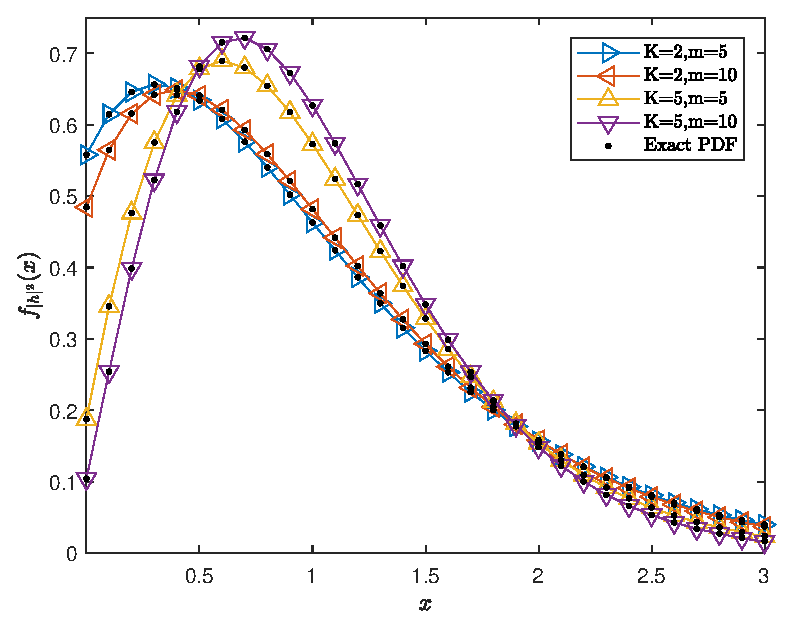
\includegraphics [width=0.45\columnwidth]{chap5_fig/pdf_comparison.eps} 
%\vspace{-0.5cm}
\caption{Comparison between the exact PDF of $|h|^2$ and power series approximation equivalent for $\Omega=1$ and $K_{tr}=50$.}
%\vspace{-0.2cm}
\label{fig:HBD_UCS_Rician_Shadowed_pdf_comparison}
\end{figure}

Let $\overline{a}\big(n,\Omega,K,m,\gamma\big)$ be defined as:
%%%%%%%%%%%%%%%%%%%%%%%%%%%%%%%%%%%%%%%%%%%%%%%%%%%%%%%%%%%%%%%%%%%%%%%%%%%%%%%%%
\begin{eqnarray} \label{HBD_UCS_Rician_Shadowed_rician_shad_cdf_exp}
\overline{a}\big(n,\Omega,K,m,\gamma\big) = \sum_{i=0}^n (-1)^{n-i} \bigg(\frac{m}{K+m}\bigg)^{m} \frac{(m)_i}{\Gamma^2(i+1)} \bigg(\frac{K}{K+m}\bigg)^{i} \bigg(\frac{1+K}{\Omega}\bigg)^{n+1} \frac{\gamma^{n+1}}{(n-i)!(n+1)}_.
\end{eqnarray}
%%%%%%%%%%%%%%%%%%%%%%%%%%%%%%%%%%%%%%%%%%%%%%%%%%%%%%%%%%%%%%%%%%%%%%%%%%%%%%%%%
Then, alternative power series representations of the Rician shadowed fading PDF and the corresponding CDF are presented as follows.

\begin{theorem} \label{HBD_UCS_Rician_Shadowed_pdf_theorem}
The PDF of $|h|^2$ can be represented as the following power series:
%%%%%%%%%%%%%%%%%%%%%%%%%%%%%%%%%%%%%%%%%%%%%%%%%%%%%%%%%%%%%%%%%%%%%%%%%%%%%%%%%
\begin{eqnarray} \label{HBD_UCS_Rician_Shadowed_rician_shad_pdf_pwr_srs}
f_{|h|^2}(x) \approx \sum_{n=0}^{K_{tr}} \overline{a}\big(n,\Omega,K,m,1\big)(n+1)x^n,
\end{eqnarray}
%%%%%%%%%%%%%%%%%%%%%%%%%%%%%%%%%%%%%%%%%%%%%%%%%%%%%%%%%%%%%%%%%%%%%%%%%%%%%%%%%
where $K_{tr}$ denotes the truncation order.
\end{theorem}
\begin{proof} 
The proof can be found in \cite{tan2018ricianShad} and is reproduced in Appendix \ref{HBD_UCS_Rician_Shadowed_pdf_theorem_proof}.
\end{proof}

\begin{theorem} \label{HBD_UCS_Rician_Shadowed_cdf_theorem}
The CDF of $|h|^2$ can be expressed as the following power series: 
%%%%%%%%%%%%%%%%%%%%%%%%%%%%%%%%%%%%%%%%%%%%%%%%%%%%%%%%%%%%%%%%%%%%%%%%%%%%%%%%%
\begin{eqnarray} \label{HBD_UCS_Rician_Shadowed_rician_shad_cdf_pwr_srs}
F_{|h|^2}(\gamma) = \int^{\gamma}_0 f_{|h|^2}(x) dx  \approx  \sum_{n=0}^{K_{tr}} \overline{a}\big(n,\Omega,K,m,\gamma\big)_.
\end{eqnarray}
%%%%%%%%%%%%%%%%%%%%%%%%%%%%%%%%%%%%%%%%%%%%%%%%%%%%%%%%%%%%%%%%%%%%%%%%%%%%%%%%%
\end{theorem}
\begin{proof}
The CDF is obtained by interchanging the summation and integration, i.e., term-wise integration \cite{gradshteyn2014table}.
\end{proof}

\begin{theorem} \label{HBD_UCS_Rician_Shadowed_l_moment_theorem}
The $l^{th}$ moment of $|h|^2$ is given as \cite[eq. (10)]{chun2017comprehensive}:
%%%%%%%%%%%%%%%%%%%%%%%%%%%%%%%%%%%%%%%%%%%%%%%%%%%%%%%%%%%%%%%%%%%%%%%%%%%%%%%%%
\begin{eqnarray} \label{HBD_UCS_Rician_Shadowed_rician_shad_frac_moment}
E\big\{\big(|h|^2\big)^l\big\} & = & \bigg(\frac{\Omega}{1+K}\bigg)^l \Gamma(1+l) \bigg(\frac{m}{K+m}\bigg)^{m-1-l} {}_2F_1\bigg(1-m,1+l;1;\frac{-K}{m}\bigg)_,
\end{eqnarray}
%%%%%%%%%%%%%%%%%%%%%%%%%%%%%%%%%%%%%%%%%%%%%%%%%%%%%%%%%%%%%%%%%%%%%%%%%%%%%%%%%
where $_2F_1(\bullet)$ is the Gauss hypergeometric function \cite{kumar2015approximate}. 
\end{theorem}

Fig. \ref{fig:HBD_UCS_Rician_Shadowed_pdf_comparison} shows the power series representation of $f_{|h|^2}(x)$, computed from (\ref{HBD_UCS_Rician_Shadowed_rician_shad_pdf_pwr_srs}), with the exact PDF in (\ref{HBD_UCS_Rician_Shadowed_rician_shad_pdf}) plotted for comparison. It can be seen that (\ref{HBD_UCS_Rician_Shadowed_rician_shad_pdf_pwr_srs}) provides a close fit to the exact PDF at the cost of computation time, which increases as $m\to\infty$. \textcolor{black}{\footnote{\textcolor{black}{To analytically gauge the accuracy of the new power series expressions, one will need to conduct a truncation analysis. Work in this direction is left as an open research challenge which can be addressed in future studies.}}} Additionally, although not plotted in Fig. \ref{fig:HBD_UCS_Rician_Shadowed_pdf_comparison}, one obtains the Rician fading PDF by letting $m \to \infty$.
 
The closed-form expressions of the PDF, CDF and fractional moments of $|h|^2$, given in (\ref{HBD_UCS_Rician_Shadowed_rician_shad_pdf_pwr_srs}), (\ref{HBD_UCS_Rician_Shadowed_rician_shad_cdf_pwr_srs}), and (\ref{HBD_UCS_Rician_Shadowed_rician_shad_frac_moment}), respectively, are useful in evaluating performance metrics, such as outage probability, in shadowing environments. \textcolor{black}{Furthermore, the new power series expressions for the PDF, CDF and frational moments are, to the best of our knowledge, not available in the literature.}

\subsection{Rician Fading Model}
To understand the impact of shadowing, (\ref{HBD_UCS_Rician_Shadowed_rician_shad_cdf_exp}) and (\ref{HBD_UCS_Rician_Shadowed_rician_shad_frac_moment}) can be evaluated for large values of $m$. In particular, one obtains the Rician fading channel $h^{'}$ from the Rician shadowed fading channel $h$ as $m \to \infty$. In the following Corollaries, new closed-form expressions for Rician fading models are presented.

\begin{corollary} \label{HBD_UCS_Rician_Shadowed_rician_fading_alpha_corollary}
As $m \to \infty$, (\ref{HBD_UCS_Rician_Shadowed_rician_shad_cdf_exp}) can be expressed as:
%%%%%%%%%%%%%%%%%%%%%%%%%%%%%%%%%%%%%%%%%%%%%%%%%%%%%%%%%%%%%%%%%%%%%%%%%%%%%%%%%
\begin{eqnarray} \label{rician_fading_alpha}
\widehat{a}\big(n,\Omega,K,\gamma\big) = \sum_{i=0}^n \frac{(-1)^{n-i} K^i}{\Gamma^2(i+1)} \bigg(\frac{1+K}{\Omega}\bigg)^{n+1} \frac{\exp(-K)\gamma^{n+1}}{(n-i)!(n+1)}_.
\end{eqnarray}
%%%%%%%%%%%%%%%%%%%%%%%%%%%%%%%%%%%%%%%%%%%%%%%%%%%%%%%%%%%%%%%%%%%%%%%%%%%%%%%%%
\end{corollary}
\begin{proof}
The proof can be found in Appendix \ref{HBD_UCS_Rician_Shadowed_rician_fading_alpha_corollary_proof}.
\end{proof}

\begin{remark}
Although not shown in Corollary \ref{HBD_UCS_Rician_Shadowed_rician_fading_alpha_corollary}, it should be noted that \textcolor{black}{the value in }$\widehat{a}\big(n,\Omega,K,\gamma\big)$ in (\ref{rician_fading_alpha}) reduces as $K \to \infty$.
\end{remark}

\begin{corollary} \label{HBD_UCS_Rician_Shadowed_rician_pdf_cdf_corollary}
The PDF $\big(f_{|h^{'}|^2}(\bullet)\big)$ and CDF $\big(F_{|h^{'}|^2}(\bullet)\big)$ of the Rician fading channel $h^{'}$ can be represented as the following power series:
%%%%%%%%%%%%%%%%%%%%%%%%%%%%%%%%%%%%%%%%%%%%%%%%%%%%%%%%%%%%%%%%%%%%%%%%%%%%%%%%%
\begin{eqnarray}
f_{|h^{'}|^2}(x) & \approx & \sum_{n=0}^{K_{tr}} \widehat{a}\big(n,\Omega,K,1\big)(n+1){x^n}_, \label{HBD_UCS_Rician_Shadowed_rician_pdf} \\
F_{|h^{'}|^2}(\gamma) & \approx & \sum_{n=0}^{K_{tr}} \widehat{a}\big(n,\Omega,K,\gamma\big)_, \label{HBD_UCS_Rician_Shadowed_rician_cdf}
\end{eqnarray}
%%%%%%%%%%%%%%%%%%%%%%%%%%%%%%%%%%%%%%%%%%%%%%%%%%%%%%%%%%%%%%%%%%%%%%%%%%%%%%%%%
where $\widehat{a}\big(n,\Omega,K,\gamma\big)$ is given in (\ref{rician_fading_alpha}).
\end{corollary}
\begin{proof}
From (\ref{rician_fading_alpha}), algebraic manipulation yields the power series expression of $f_{|h^{'}|^2}(\bullet)$ and $F_{|h^{'}|^2}(\bullet)$ in (\ref{HBD_UCS_Rician_Shadowed_rician_pdf}) and (\ref{HBD_UCS_Rician_Shadowed_rician_cdf}), respectively.
\end{proof}

\begin{corollary} \label{HBD_UCS_Rician_Shadowed_frac_moments_corollary}
The closed-form expression for the $l^{th}$ moment of $|h^{'}|^2$ is: 
%%%%%%%%%%%%%%%%%%%%%%%%%%%%%%%%%%%%%%%%%%%%%%%%%%%%%%%%%%%%%%%%%%%%%%%%%%%%%%%%%
\begin{eqnarray} \label{HBD_UCS_Rician_Shadowed_frac_moments_corollary_comp_limits}
E\big\{\big(|h^{'}|^2\big)^{l}\big\} = \lim_{m\to\infty}E\big\{\big(|h|^2\big)^l\big\} \approx \bigg(\frac{\Omega}{1+K}\bigg)^l \Gamma(1+l) \sum_{n=0}^{K_{tr}} \frac{(-l)_n}{n!(1)_n}{(-K)^n}_.
\end{eqnarray}
%%%%%%%%%%%%%%%%%%%%%%%%%%%%%%%%%%%%%%%%%%%%%%%%%%%%%%%%%%%%%%%%%%%%%%%%%%%%%%%%%
\end{corollary}
\begin{proof}
The proof can be found in Appendix \ref{HBD_UCS_Rician_Shadowed_frac_moments_corollary_proof}.
\end{proof}

\begin{figure} [t]
\centering
\vspace{0.2cm}
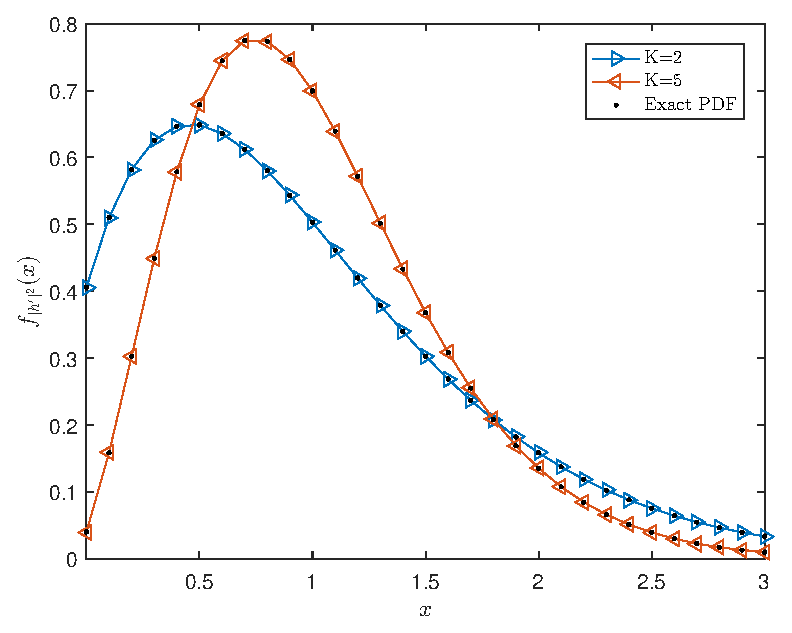
\includegraphics [width=0.45\columnwidth]{chap5_fig/alt_pdf_comparison.eps} 
%\vspace{-0.5cm}
\caption{Comparison between the exact PDF of $|h^{'}|^2$ and power series approximation equivalent for $\Omega=1$ and $K_{tr}=50$.}
%\vspace{-0.2cm}
\label{fig:HBD_UCS_Rician_Shadowed_alt_pdf_comparison}
\end{figure}

\begin{figure} [t]
\centering
\vspace{0.2cm}
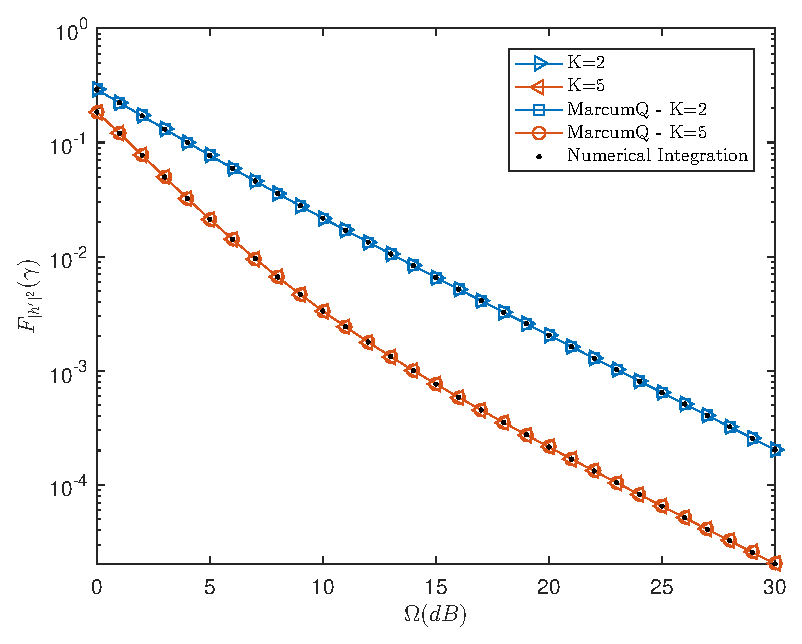
\includegraphics [width=0.45\columnwidth]{chap5_fig/alt_cdf_comparison.eps} 
%\vspace{-0.5cm}
\caption{Comparison between the exact CDF of $|h^{'}|^2$ and power series approximation equivalent for $\gamma=0.5$ and $K_{tr}=50$.}
%\vspace{-0.2cm}
\label{fig:HBD_UCS_Rician_Shadowed_alt_cdf_comparison}
\end{figure}

\begin{figure} [t]
\centering
\vspace{0.2cm}
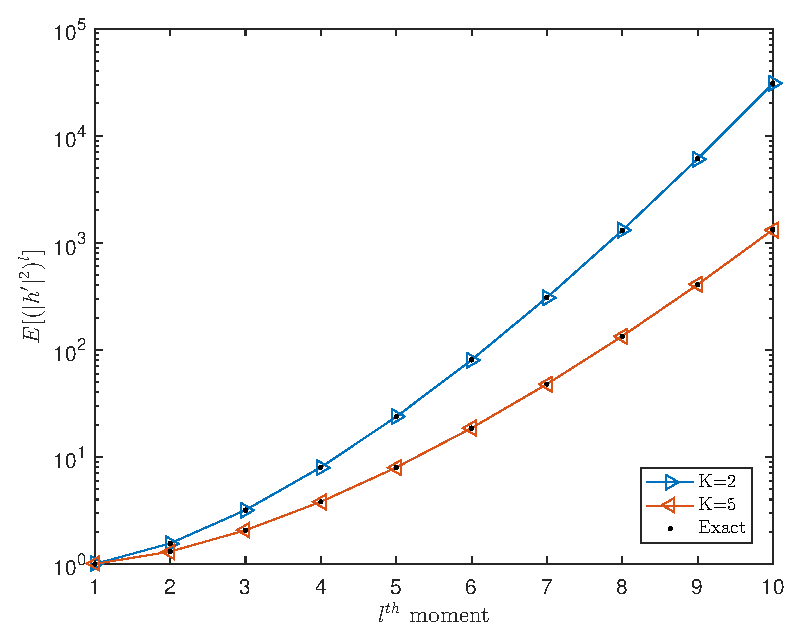
\includegraphics [width=0.45\columnwidth]{chap5_fig/alt_moment_comparison.eps} 
%\vspace{-0.5cm}
\caption{Comparison between the exact fractional moment of $|h^{'}|^2$ and power series approximation equivalent for $\Omega=1$ and $K_{tr}=50$.}
%\vspace{-0.2cm}
\label{fig:HBD_UCS_Rician_Shadowed_alt_moment_comparison}
\end{figure}

The Rician fading PDF in (\ref{HBD_UCS_Rician_Shadowed_rician_pdf}) is plotted in Fig. \ref{fig:HBD_UCS_Rician_Shadowed_alt_pdf_comparison} and compared against the exact Rician fading PDF $f_{|h^{'}|^2}(x) = \frac{K+1}{\Omega} \exp\left(-K-\frac{K+1}{\Omega}x\right)I_{0}\left(2\sqrt{\frac{K(K+1)}{\Omega}x}\right)$, where $I_{0}\left(\cdot\right)$ is the modified Bessel function of the first kind with zero order \cite{gradshteyn2014table}. It can be observed that (\ref{HBD_UCS_Rician_Shadowed_rician_pdf}) provides a close fit to the exact PDF in Fig. \ref{fig:HBD_UCS_Rician_Shadowed_alt_pdf_comparison}. 

The Rician fading CDF $F_{|h^{'}|^2}(\gamma)$ in (\ref{HBD_UCS_Rician_Shadowed_rician_cdf}) is plotted in Fig. \ref{fig:HBD_UCS_Rician_Shadowed_alt_cdf_comparison}. When compared against the numerical integration of $f_{|h^{'}|^2}(x)$ and the exact CDF, $F_{|h^{'}|^2}(\gamma)=1- \\ Q_1\Big( \sqrt{2K}, \sqrt{\frac{2(K+1)\gamma}{\Omega}}\Big)$ where $Q_1\left(\cdot,\cdot\right)$ is the Marcum Q function \cite{rached2017unified}, a close fit is also observed. Similar observations are also made in Fig. \ref{fig:HBD_UCS_Rician_Shadowed_alt_moment_comparison} when (\ref{HBD_UCS_Rician_Shadowed_frac_moments_corollary_comp_limits}) is compared against $E\big\{\big(|h^{'}|^2\big)^l\big\} = \Gamma(1+l) \left[\frac{\Omega}{1+K}\right]^{l} {}_1{F_1}(-l,1;-K)$ \cite[Table II]{rached2017unified}.

Evidently, (\ref{HBD_UCS_Rician_Shadowed_rician_shad_cdf_exp}) and (\ref{HBD_UCS_Rician_Shadowed_rician_shad_frac_moment}) become independent of $m$ as $m \to \infty$. More importantly, Corollaries \ref{HBD_UCS_Rician_Shadowed_rician_fading_alpha_corollary} and \ref{HBD_UCS_Rician_Shadowed_frac_moments_corollary} show that the computed values of (\ref{HBD_UCS_Rician_Shadowed_rician_shad_cdf_exp}) and (\ref{HBD_UCS_Rician_Shadowed_rician_shad_frac_moment}) decreases and increases, respectively, based on the Rician $K$ factor as $m \to \infty$. The presented power series representations of the Rician shadowed fading and Rician fading models in this section are summarized in Table \ref{table:HBD_UCS_Rician_Shadowed_summary_statistics}\footnote{The functions $\gamma(\cdot,\cdot)$, $I_{0}\left(\cdot\right)$, $Q_1\left(\cdot,\cdot\right)$, and ${}_1{F_1}(\bullet)$ represent the lowercase incomplete gamma function \cite{chun2017comprehensive}, the modified Bessel function of the first kind with zero order \cite{gradshteyn2014table}, the Marcum Q function \cite{rached2017unified}, and the confluent Hypergeometric function \cite{gradshteyn2014table}, respectively. The fractional moment of $|h|^2$, i.e., $E\{(|h|^2)^j\}$ is given in (\ref{HBD_UCS_Rician_Shadowed_rician_shad_frac_moment}) while $\overline{a}\big(n,\Omega,K,m,1\big)$ and $\widehat{a}\big(n,\Omega,K,\gamma\big)$ are given in (\ref{HBD_UCS_Rician_Shadowed_rician_shad_cdf_exp}) and (\ref{rician_fading_alpha}), respectively.}. Together, these observations and expressions are essential in evaluating the outage probability of the HBD-UCS, which is discussed in Section \ref{HBD_UCS_Rician_Shadowed_sec_outage}.

%\begin{table*}[]
%\centering
%\caption{Summary of presented closed-form expressions for the Rician shadowed fading and Rician fading models}
%\label{table:HBD_UCS_Rician_Shadowed_summary_statistics}
%\scalebox{0.7}{
%\begin{tabular}{lll}
%\hline
%\textbf{Fading Model}	& \textbf{Expression}																																																											& \textbf{Comment}	\\ \hline \hline
%Rician shadowed (PDF)	& $f_{|h|^2}(x) \approx \sum_{n=0}^{K_{tr}} \overline{a}\big(n,\Omega,K,m,1\big)(n+1)x^n$ 																								& Current Work 							\\
											%& $f_{|h|^2}(x) = \frac{m^m (1+K)}{\Omega(K+m)^m}\exp\Big(\frac{-(1+K)x}{\Omega}\Big){}_1F_1\Big(m;1;\frac{K(1+K)x}{(K+m)\Omega}\Big)$		& \cite{chun2017comprehensive} \\
											%& $f_{|h|^2}(x) = \sum_{n=0}^{\infty} \sum_{i=0}^{n} \sum_{j=0}^{n} \frac{(-1)^{i+j}}{\Gamma[i+1]j!}\binom{n}{i} \binom{n}{n-j} E\{(|h|^2)^j\}x^{i}\exp(-x)$ 																																																																																& \cite{chun2017comprehensive} \\
%Rician shadowed	(CDF)	& $F_{|h|^2}(\gamma) \approx  \sum_{n=0}^{K_{tr}} \overline{a}\big(n,\Omega,K,m,\gamma\big)$ 																							& Current Work 							\\
											%& $F_{|h|^2}(x) = \sum_{n=0}^{\infty} \sum_{i=0}^{n} \sum_{j=0}^{n} \frac{(-1)^{i+j}}{\Gamma(i+2)j!} \binom{n}{i} \binom{n}{n-j} E\{(|h|^2)^j\}x^{i+1} + \gamma(1,x)$ 																																																																															 & \cite{chun2017comprehensive} \\
%Rician (PDF)					& $f_{|h^{'}|^2}(x) \approx \sum_{n=0}^{K_{tr}} \widehat{a}\big(n,\Omega,K,1\big)(n+1)x^n$ 																								& Current Work 							\\
											%&	$f_{|h^{'}|^2}(x) = \frac{K+1}{\Omega} \exp\left(-K-\frac{K+1}{\Omega}x\right)I_{0}\left(2\sqrt{\frac{K(K+1)}{\Omega}x}\right)$ 				& \cite{rached2017unified} 	\\
%Rician (CDF)					& $F_{|h^{'}|^2}(\gamma) \approx \sum_{n=0}^{K_{tr}} \widehat{a}\big(n,\Omega,K,\gamma\big)$ 																							& Current Work 						 	\\ 
											%&	$F_{|h^{'}|^2}(\gamma)=1-Q_1\Big( \sqrt{2K}, \sqrt{\frac{2(K+1)\gamma}{\Omega}}\Big)$ 																									& \cite{rached2017unified} 	\\
%Rician (Fractional Moment)	& $E\big\{\big({|h^{'}|^2}\big)^l\big\} \approx \Big(\frac{\Omega}{1+K}\Big)^l \Gamma(1+l) \sum_{n=0}^{K_{tr}} \frac{(-l)_n}{n!(1)_n}(-K)^n$ & Current Work 					\\
											%&	$E\big\{\big({|h^{'}|^2}\big)^l\big\} = \Gamma(1+l) \left[\frac{\Omega}{1+K}\right]^{l} {}_1{F_1}(-l,1;-K)$ 														& \cite{rached2017unified} 	\\ \hline
%\end{tabular}}
%\end{table*}

\begin{table*}[]
\centering
\caption{Summary of presented closed-form expressions for the Rician shadowed fading and Rician fading models}
\label{table:HBD_UCS_Rician_Shadowed_summary_statistics}
\scalebox{0.8}{
\begin{tabular}{lll}
\hline
\textbf{Fading Model}	& \textbf{PDF Expression}																																																									& \textbf{Comment}	\\ \hline \hline
Rician shadowed 			& $f_{|h|^2}(x) \approx \sum_{n=0}^{K_{tr}} \overline{a}\big(n,\Omega,K,m,1\big)(n+1)x^n$ 																								& Current Work 							\\
											& $f_{|h|^2}(x) = \frac{m^m (1+K)}{\Omega(K+m)^m}\exp\Big(\frac{-(1+K)x}{\Omega}\Big){}_1F_1\Big(m;1;\frac{K(1+K)x}{(K+m)\Omega}\Big)$		& \cite{chun2017comprehensive} \\
											& $f_{|h|^2}(x) = \sum_{n=0}^{\infty} \sum_{i=0}^{n} \sum_{j=0}^{n} \frac{(-1)^{i+j}}{\Gamma[i+1]j!}\binom{n}{i} \binom{n}{n-j} E\{(|h|^2)^j\}x^{i}\exp(-x)$ 																																																																																& \cite{chun2017comprehensive} \\
Rician 								& $f_{|h^{'}|^2}(x) \approx \sum_{n=0}^{K_{tr}} \widehat{a}\big(n,\Omega,K,1\big)(n+1)x^n$ 																								& Current Work 							\\
											&	$f_{|h^{'}|^2}(x) = \frac{K+1}{\Omega} \exp\left(-K-\frac{K+1}{\Omega}x\right)I_{0}\left(2\sqrt{\frac{K(K+1)}{\Omega}x}\right)$ 				& \cite{rached2017unified} 	\\
											&																																																																					& 													\\	\hline
\textbf{Fading Model}	& \textbf{CDF Expression}																																																									& \textbf{Comment}					\\ \hline \hline
Rician shadowed				& $F_{|h|^2}(\gamma) \approx  \sum_{n=0}^{K_{tr}} \overline{a}\big(n,\Omega,K,m,\gamma\big)$ 																							& Current Work 							\\
											& $F_{|h|^2}(x) = \sum_{n=0}^{\infty} \sum_{i=0}^{n} \sum_{j=0}^{n} \frac{(-1)^{i+j}}{\Gamma(i+2)j!} \binom{n}{i} \binom{n}{n-j} E\{(|h|^2)^j\}x^{i+1} + \gamma(1,x)$ 																																																																															 & \cite{chun2017comprehensive} \\
Rician 								& $F_{|h^{'}|^2}(\gamma) \approx \sum_{n=0}^{K_{tr}} \widehat{a}\big(n,\Omega,K,\gamma\big)$ 																							& Current Work 						 	\\ 
											&	$F_{|h^{'}|^2}(\gamma)=1-Q_1\Big( \sqrt{2K}, \sqrt{\frac{2(K+1)\gamma}{\Omega}}\Big)$ 																									& \cite{rached2017unified} 	\\
											&																																																																					&														\\ \hline
\textbf{Fading Model}	& \textbf{Fractional Moments Expression}																																																	& \textbf{Comment}					\\ \hline \hline
Rician 								& $E\big\{\big({|h^{'}|^2}\big)^l\big\} \approx \Big(\frac{\Omega}{1+K}\Big)^l \Gamma(1+l) \sum_{n=0}^{K_{tr}} \frac{(-l)_n}{n!(1)_n}(-K)^n$ & Current Work 					\\
											&	$E\big\{\big({|h^{'}|^2}\big)^l\big\} = \Gamma(1+l) \left[\frac{\Omega}{1+K}\right]^{l} {}_1{F_1}(-l,1;-K)$ 														& \cite{rached2017unified} 	\\ \hline
\end{tabular}}
\end{table*}


%\begin{sidewaystable}[]
%\centering
%\caption{Summary of presented closed-form expressions for the Rician shadowed fading and Rician fading models}
%\label{table:HBD_UCS_Rician_Shadowed_summary_statistics}
%\scalebox{0.7}{
%\begin{tabular}{cccc}
%\hline
%\textbf{Fading Model}	& \textbf{Power Series Representation (Current Work)}		& \textbf{State-of-the-Art }	& \textbf{Reference} \\ \hline \hline
%Rician shadowed				& $f_{|h|^2}(x) \approx \sum_{n=0}^{K_{tr}} \overline{a}\big(n,\Omega,K,m,1\big)(n+1)x^n$ & $f_{|h|^2}(x) = \frac{m^m (1+K)}{\Omega(K+m)^m}\exp\Big(\frac{-(1+K)x}{\Omega}\Big){}_1F_1\Big(m;1;\frac{K(1+K)x}{(K+m)\Omega}\Big)$  & \cite{chun2017comprehensive} \\
 %&  & $f_{|h|^2}(x) = \sum_{n=0}^{\infty} \sum_{i=0}^{n} \sum_{j=0}^{n} \frac{(-1)^{i+j}}{\Gamma[i+1]j!}\binom{n}{i} \binom{n}{n-j} E\{(|h|^2)^j\}x^{i}\exp(-x)$ & \cite{chun2017comprehensive} \\
%Rician shadowed & $F_{|h|^2}(\gamma) \approx  \sum_{n=0}^{K_{tr}} \overline{a}\big(n,\Omega,K,m,\gamma\big)$ & \hspace{-0.4cm} $F_{|h|^2}(x) = \sum_{n=0}^{\infty} \sum_{i=0}^{n} \sum_{j=0}^{n} \frac{(-1)^{i+j}}{\Gamma(i+2)j!} \binom{n}{i} \binom{n}{n-j} E\{(|h|^2)^j\}x^{i+1} + \gamma(1,x)$ & \cite{chun2017comprehensive} \\
%Rician & $f_{|h^{'}|^2}(x) \approx \sum_{n=0}^{K_{tr}} \widehat{a}\big(n,\Omega,K,1\big)(n+1)x^n$ & $f_{|h^{'}|^2}(x) = \frac{K+1}{\Omega} \exp\left(-K-\frac{K+1}{\Omega}x\right)I_{0}\left(2\sqrt{\frac{K(K+1)}{\Omega}x}\right)$ & \cite{rached2017unified} \\
%Rician & $F_{|h^{'}|^2}(\gamma) \approx \sum_{n=0}^{K_{tr}} \widehat{a}\big(n,\Omega,K,\gamma\big)$ & $F_{|h^{'}|^2}(\gamma)=1-Q_1\Big( \sqrt{2K}, \sqrt{\frac{2(K+1)\gamma}{\Omega}}\Big)$ & \cite{rached2017unified} \\
%Rician & $E\big\{\big({|h^{'}|^2}\big)^l\big\} \approx \Big(\frac{\Omega}{1+K}\Big)^l \Gamma(1+l) \sum_{n=0}^{K_{tr}} \frac{(-l)_n}{n!(1)_n}(-K)^n$ & $E\big\{\big({|h^{'}|^2}\big)^l\big\} = \Gamma(1+l) \left[\frac{\Omega}{1+K}\right]^{l} {}_1{F_1}(-l,1;-K)$ & \cite{rached2017unified} \\
 %& & & \\ \hline
%\end{tabular}}
%\end{sidewaystable}
  
%%%%%%%%%%%%%%%%%%%%%%%%%%%%%%%%%%%%%%%%%%%%%%%%%%%%%%%%%%%%%%%%%%%%%%%%%%%%%%%%%%%%%%%%%%%%%%%%%%%%%%%%%%%%%%%%%%%%%%%%%%%%%%%%%%%%%%%%%
% Section 4 : Outage Probability Derivations
\section{Outage Probability Derivations} \label{HBD_UCS_Rician_Shadowed_sec_outage}
In this section, closed-form outage probability expressions are derived for the HBD-UCS. The transmission rates of UAV-1 and GS are defined as $R^{HBD}_{1}$ and $R^{HBD}_{gs}$, respectively, with HBD system sum rate defined as $R^{HBD}_{sum} = R^{HBD}_{1}+R^{HBD}_{gs}$. Similarly for HD transmission, the transmission rates of UAV-1 and GS are defined as $R^{HD}_{1}$ and $R^{HD}_{gs}$, respectively, with HD system sum rate $R^{HD}_{sum} = R^{HD}_{1}+R^{HD}_{gs}$. To maintain a fair comparison between HBD and HD systems, we let $R_{i}^{HBD}=\frac{1}{2}R_{i}^{HD}$ for $ i \in \{1, gs\}$ \cite{sofotasios2017full}. Based on these definitions, the HBD and HD outage probabilities at GS and UAV-2 are defined in the following subsections.

%%%%%%%%%%%%%%%%%%%%%%%%%%%%%%%%%%%%%%%%%%%%%%%%%%%%%%%%%%%%%%%%%%%%%%%%%%%%%%%%%%%%%%%%%%%%%%%%%%%%%%%%%%%%%%%%%%%%%%%%%%%%%%%%%%%%%%%%%%
\subsection{Hybrid-Duplex Outage Probability}
% introduce the RVs for GS outage probability expression
Starting with the FD-enabled GS, strong SI is experienced due to the simultaneous transmission and reception of $x_{gs}[t]$ and $x_1[t]$, respectively. Let the instantaneous received signal power of the SOI at GS be $X_{1}=\Omega_X|h_{1,g}|^2$, modeled as a Rician shadowed distributed RV with Rician $K$ factor $K_{X_{1}}$ and shadowing severity parameter $m_{X_{1}}$. Also, let the instantaneous received signal power of the SI components be $Y_{si,1}=\Omega_X\alpha_{g,g}\gamma_{\phi}^2|h_{si}|^2$ and $Y_{si,2}=\Omega_X\alpha_{g,g}\epsilon|\widetilde{h}_{si}|^2$. The RVs, $Y_{si,1}$ and $Y_{si,2}$, are modeled as a Rician shadowed distributed RV with Rician $K$ factor $K_{Y_{si,1}}$ and shadowing parameter $m_{Y_{si,1}}$, and an exponentially distributed RV, respectively.

% introduce the RVs for UAV-2 outage probability expression
At UAV-2, let the instantaneous received signal power of the SOI and interference be $X_{gs} = \Omega_{X}\alpha_{g,2}|h_{g,2}|^2$ and $Y_{1}=\Omega_{X}\alpha_{1,2}|h_{1,2}|^2$, respectively. Both $X_{gs}$ and $Y_{1}$ are respectively modeled as independent Rician shadowed distributed RVs, with Rician $K$ factors $K_{X_{gs}}$ and $K_{Y_1}$, and shadowing severity parameters $m_{X_{gs}}$ and $m_{Y_1}$.

% Outage probability at GS
\subsubsection{Ground Station}
At the FD-enabled GS, SI mitigation is imperfect due to phase noise and SI channel estimation error. As a result, residual SI is experienced at the GS. Thus, an II detector is assumed at the GS, which treats residual SI ($Y_{si,1},Y_{si,2}$) as noise when detecting the SOI ($X_1$). Let the outage event, outage probability, and the HBD threshold at the FD-enabled GS be $\mathcal{O}_{gs}^{HBD} = \Big\{ h_{1,g}, h_{si}, \widetilde{h}_{si}: R_{1}^{HBD} \geq \log_{2}\Big(1 + \frac{X_{1}}{Y_{si,1} + Y_{si,2} + 1}\Big)\Big\}$, $Pr\big(\mathcal{O}_{gs}^{HBD}\big)$, and $\gamma_{th,gs}^{HBD} = 2^{R_{1}^{HBD}}-1$, respectively.

\begin{theorem} \label{HBD_UCS_Rician_Shadowed_P_out_gs_theorem}
The closed-form outage probability at GS over Rician shadowed fading channels is:
%%%%%%%%%%%%%%%%%%%%%%%%%%%%%%%%%%%%%%%%%%%%%%%%%%%%%%%%%%%%%%%%%%%%%%%%%%%%%%%%%
\begin{eqnarray} \label{HBD_UCS_Rician_Shadowed_P_out_GS_HBD}
Pr\big(\mathcal{O}_{gs}^{HBD}\big) \approx \sum_{n=0}^{K_{tr}} \sum_{l_1 + l_2 + l_3 = n+1} \overline{a}\big(n,\Omega_X,K_{X_1},m_{X_1},\gamma_{th,gs}^{HBD}\big) \frac{(n+1)!}{l_1! \cdot l_2! \cdot l_3!} E\{Y_{si,1}^{l_1}\} E\{Y_{si,2}^{l_2}\}_,
\end{eqnarray}
%%%%%%%%%%%%%%%%%%%%%%%%%%%%%%%%%%%%%%%%%%%%%%%%%%%%%%%%%%%%%%%%%%%%%%%%%%%%%%%%%
where
%%%%%%%%%%%%%%%%%%%%%%%%%%%%%%%%%%%%%%%%%%%%%%%%%%%%%%%%%%%%%%%%%%%%%%%%%%%%%%%%%
\begin{eqnarray}
E\{Y_{si,1}^{l_1}\} & = & \Gamma(1+l_1) \bigg(\frac{\alpha_{g,g}\gamma_{\phi}^2}{1+K_{Y_{si,1}}}\bigg)^{l_1} \bigg(\frac{m_{Y_{si,1}}}{K_{Y_{si,1}}+m_{Y_{si,1}}}\bigg)^{m_{Y_{si,1}}-1-l_1} \nonumber\\
 & & \hspace{3cm} \times {}_2F_1\bigg(1-m_{Y_{si,1}},1+l_1;1;\frac{-K_{Y_{si,1}}}{m_{Y_{si,1}}}\bigg) {\big(\Omega_X\big)^{l_1}}_, \\
E\{Y_{si,2}^{l_2}\} & = & \Gamma(1+l_2) (\alpha_{g,g}\epsilon\big)^{l_2} {(\Omega_X)^{l_2}}_.
\end{eqnarray}
%%%%%%%%%%%%%%%%%%%%%%%%%%%%%%%%%%%%%%%%%%%%%%%%%%%%%%%%%%%%%%%%%%%%%%%%%%%%%%%%%
\end{theorem}
\begin{proof}
The outage probability at GS can be obtained as $Pr\big(\mathcal{O}_{gs}^{HBD}\big) = E\Big\{F_{X_{1}}\Big( \gamma_{th,gs}^{HBD}(1+Y_{si,1}+Y_{si,2}) \Big)\Big\}$, where $F_{X_{1}}(\bullet)$ is the CDF of $X_1$ obtained from (\ref{HBD_UCS_Rician_Shadowed_rician_shad_cdf_pwr_srs}). The final expression for $Pr\big(\mathcal{O}_{gs}^{HBD}\big)$ can be calculated from \cite[eq. (8)]{rached2017unified}, with the proof of convergence given in Appendix \ref{HBD_UCS_Rician_Shadowed_P_out_GS_HBD_conv}.\end{proof}

As shadowing is considered at the GS, the impact of shadowing on the SI link due to passive SI suppression can be investigated using (\ref{HBD_UCS_Rician_Shadowed_P_out_GS_HBD}). Furthermore, for the case of Rician fading channels, we present an alternative outage probability expression from (\ref{HBD_UCS_Rician_Shadowed_P_out_GS_HBD}) in the following Corollary.

\begin{corollary} \label{HBD_UCS_Rician_Shadowed_corollary_P_out_GS_HBD_rician}
The closed-form outage probability at GS over Rician fading channels is:
%%%%%%%%%%%%%%%%%%%%%%%%%%%%%%%%%%%%%%%%%%%%%%%%%%%%%%%%%%%%%%%%%%%%%%%%%%%%%%%%%
\begin{eqnarray} \label{HBD_UCS_Rician_Shadowed_P_out_GS_HBD_rician}
Pr\big(\mathcal{O}_{gs}^{HBD*}\big) & \approx & \sum_{n=0}^{K_{tr}} \sum_{l_1 + l_2 + l_3 = n+1} \widehat{a}\big(n,\Omega_X,K_{X_1},\gamma_{th,gs}^{HBD}\big) \frac{(n+1)!}{l_1! \cdot l_2! \cdot l_3!} E\{Y_{si,1}^{l_1*}\} E\{Y_{si,2}^{l_2}\}_,
\end{eqnarray}
%%%%%%%%%%%%%%%%%%%%%%%%%%%%%%%%%%%%%%%%%%%%%%%%%%%%%%%%%%%%%%%%%%%%%%%%%%%%%%%%%
where $Y_{si,1}^{l_1*}$ is a RV defined using the Rician fading model and
%%%%%%%%%%%%%%%%%%%%%%%%%%%%%%%%%%%%%%%%%%%%%%%%%%%%%%%%%%%%%%%%%%%%%%%%%%%%%%%%%
\begin{eqnarray}
\hspace{-0.25cm} E\{Y_{si,1}^{l_1*}\}  & \hspace{-0.25cm} = & \hspace{-0.25cm} \Gamma(1+l_1) \bigg(\frac{\alpha_{g,g}\gamma_{\phi}^2\Omega_X}{1+K_{Y_{si,1}}}\bigg)^{l_1} \sum_{i=0}^{K_{tr}} \frac{(-l_1)_i}{i!(1)_i}{(-K_{Y_{si,1}})^i}_.
\end{eqnarray}
%%%%%%%%%%%%%%%%%%%%%%%%%%%%%%%%%%%%%%%%%%%%%%%%%%%%%%%%%%%%%%%%%%%%%%%%%%%%%%%%%
\end{corollary}
\begin{proof}
Replacing $\overline{a}\big(n,\Omega_X,K_{X_1},m_{X_1},\gamma_{th,gs}^{HBD}\big)$ in (\ref{HBD_UCS_Rician_Shadowed_P_out_GS_HBD}) with (\ref{rician_fading_alpha}) and applying (\ref{HBD_UCS_Rician_Shadowed_frac_moments_corollary_comp_limits}) to evaluate $E\{Y_{si,1}^{l_1*}\}$ yields (\ref{HBD_UCS_Rician_Shadowed_P_out_GS_HBD_rician}). Additionally, it can be shown that (\ref{HBD_UCS_Rician_Shadowed_P_out_GS_HBD_rician}) converges absolutely by following the same steps in Appendix \ref{HBD_UCS_Rician_Shadowed_P_out_GS_HBD_conv}.
\end{proof}

The closed-form expression in Corollary \ref{HBD_UCS_Rician_Shadowed_corollary_P_out_GS_HBD_rician} \textcolor{black}{is} used as a benchmark to evaluate the reliability of the GS over Rician fading channels. From \cite{ernest2019outage}, it is known that the FD-enabled GS becomes interference-limited at high SNR regimes. Thus, in the following Corollary, the asymptotic outage probability of the FD-enabled GS over Rician shadowed fading channels and Rician fading channels is presented.

\begin{corollary} \label{HBD_UCS_Rician_Shadowed_corollary_P_out_GS_HBD_asymp}
The closed-form asymptotic outage probability expressions at the GS over Rician shadowed fading channels $\big(Pr\big(\mathcal{O}_{gs,\infty}^{HBD}\big)\big)$ and Rician fading channels $\big(Pr\big(\mathcal{O}_{gs,\infty}^{HBD*}\big)\big)$ are:
%%%%%%%%%%%%%%%%%%%%%%%%%%%%%%%%%%%%%%%%%%%%%%%%%%%%%%%%%%%%%%%%%%%%%%%%%%%%%%%%%
\begin{eqnarray} 
Pr\big(\mathcal{O}_{gs,\infty}^{HBD}\big) & \approx & \sum_{n=0}^{K_{tr}} \sum_{l_1 + l_2 = n+1} \overline{a}\big(n,1,K_{X_1},m_{X_1},\gamma_{th,gs}^{HBD}\big) \frac{(n+1)!}{l_1! \cdot l_2!} M\{Y_{si,1}^{l_1}\} M\{Y_{si,2}^{l_2}\}_, \label{HBD_UCS_Rician_Shadowed_P_out_GS_HBD_asymp} \\
Pr\big(\mathcal{O}_{gs,\infty}^{HBD*}\big) & \approx & \sum_{n=0}^{K_{tr}} \sum_{l_1 + l_2 = n+1} \widehat{a}\big(n,1,K_{X_1},\gamma_{th,gs}^{HBD}\big) \frac{(n+1)!}{l_1! \cdot l_2!} M\{Y_{si,1}^{l_1*}\} M\{Y_{si,2}^{l_2}\}_, \label{HBD_UCS_Rician_Shadowed_P_out_GS_HBD_rician_asymp}
\end{eqnarray}
%%%%%%%%%%%%%%%%%%%%%%%%%%%%%%%%%%%%%%%%%%%%%%%%%%%%%%%%%%%%%%%%%%%%%%%%%%%%%%%%%
where $M\{Z^{l}\}=E\{Z^{l}\}/(\Omega_X)^{l}$ is the normalized $l^{th}$ moment of RV $Z$ \cite{ernest2019outage}.
%%%%%%%%%%%%%%%%%%%%%%%%%%%%%%%%%%%%%%%%%%%%%%%%%%%%%%%%%%%%%%%%%%%%%%%%%%%%%%%%%
\end{corollary}
\begin{proof}
The proof is given in Appendix \ref{HBD_UCS_Rician_Shadowed_corollary_P_out_GS_HBD_asymp_proof}.
\end{proof}


As the FD-enabled GS is interference-limited \cite{ernest2019outage}, Corollary \ref{HBD_UCS_Rician_Shadowed_corollary_P_out_GS_HBD_asymp} can be used to obtain the outage probability error floor, which is useful in determining how SI and shadowing affects reliability. Further discussion on the outage probability at GS are presented in Section \ref{HBD_UCS_Rician_Shadowed_sec_num_res}.

% Outage probability at UAV-2 (II)
\subsubsection{Unmanned Aerial Vehicle 2 (Interference Ignorant Detector)}
At UAV-2, inter-UAV interference ($Y_1$) is treated as noise when the II detector is detecting the SOI ($X_{gs}$). Let the outage event, outage probability, and the HBD threshold at UAV-2 be $\mathcal{O}_{2}^{HBD(II)} = \Big\{ h_{g,2}, h_{1,2} : R_{gs}^{HBD} \geq \log_{2}\Big(1+\frac{X_{gs}}{Y_{1} + 1}\Big)\Big\}$, $Pr\big(\mathcal{O}_{2}^{HBD(II)}\big)$, and $\gamma_{th,2}^{HBD} = 2^{R_{gs}^{HBD}}-1$, respectively. 

\begin{theorem} \label{HBD_UCS_Rician_Shadowed_P_out_uav2_II_HBD_theorem}
The closed-form outage probability expression with II detector at UAV-2 over Rician shadowed fading channels is:
%%%%%%%%%%%%%%%%%%%%%%%%%%%%%%%%%%%%%%%%%%%%%%%%%%%%%%%%%%%%%%%%%%%%%%%%%%%%%%%%%
\begin{eqnarray} \label{HBD_UCS_Rician_Shadowed_P_out_uav2_II_HBD}
Pr\big(\mathcal{O}_{2}^{HBD(II)}\big) & \approx & \sum_{n=0}^{K_{tr}} \sum_{j=0}^{n+1} \overline{a}\big(n,\Omega_X\alpha_{g,2},K_{X_{gs}},m_{X_{gs}},\gamma_{th,2}^{HBD}\big) \binom{n+1}{j} E\{Y_1^{j}\}_,
\end{eqnarray}
%%%%%%%%%%%%%%%%%%%%%%%%%%%%%%%%%%%%%%%%%%%%%%%%%%%%%%%%%%%%%%%%%%%%%%%%%%%%%%%%%
where $E\{Y_1^{j}\} = \Big(\frac{\Omega_X\alpha_{1,2}}{1+K_{Y_1}}\Big)^j \Gamma(1+j) \Big(\frac{m_{Y_1}}{K_{Y_1}+m_{Y_1}}\Big)^{m_{Y_1}-1-j} {}_2F_1\Big(1-m_{Y_1},1+j;1;\frac{-K_{Y_1}}{m_{Y_1}}\Big)$.
\end{theorem}
\begin{proof}
The closed-form outage probability expression at UAV-2 can be obtained as $Pr\big(\mathcal{O}_{2}^{HBD(II)}\big) = E\Big\{F_{X_{gs}}\Big( \gamma_{th,2}^{HBD}(1+Y_1) \Big)\Big\}$, where $F_{X_{gs}}(\bullet)$ is the CDF of $X_{gs}$ from (\ref{HBD_UCS_Rician_Shadowed_rician_shad_cdf_pwr_srs}). The final expression for $Pr\big(\mathcal{O}_{2}^{HBD(II)}\big)$ is calculated from \cite[eq. (8)]{rached2017unified}. Separately, it can be shown that (\ref{HBD_UCS_Rician_Shadowed_P_out_uav2_II_HBD}) converges absolutely by repeating the same approach in Appendix \ref{HBD_UCS_Rician_Shadowed_P_out_GS_HBD_conv}.
\end{proof}

For the case of Rician fading channels, an alternative outage probability expression from (\ref{HBD_UCS_Rician_Shadowed_P_out_uav2_II_HBD}) is presented in the following Corollary.

\begin{corollary} \label{HBD_UCS_Rician_Shadowed_corollary_P_out_uav2_II_HBD_rician}
The closed-form outage probability expression with II detector at UAV-2 over Rician fading channels is:
%%%%%%%%%%%%%%%%%%%%%%%%%%%%%%%%%%%%%%%%%%%%%%%%%%%%%%%%%%%%%%%%%%%%%%%%%%%%%%%%%
\begin{eqnarray} \label{HBD_UCS_Rician_Shadowed_P_out_uav2_II_HBD_rician}
Pr\big(\mathcal{O}_{2}^{HBD(II)*}\big) & \approx & \sum_{n=0}^{K_{tr}} \sum_{j=0}^{n+1} \widehat{a}\big(n,\Omega_X\alpha_{g,2},K_{X_{gs}},\gamma_{th,2}^{HBD}\big) \binom{n+1}{j} E\{Y_1^{j*}\}_,
\end{eqnarray}
%%%%%%%%%%%%%%%%%%%%%%%%%%%%%%%%%%%%%%%%%%%%%%%%%%%%%%%%%%%%%%%%%%%%%%%%%%%%%%%%%
where $Y_1^{j*}$ is a RV defined using the Rician fading model and $E\{Y_1^{j*}\} = \Big(\frac{\Omega_X\alpha_{1,2}}{1+K_{Y_1}}\Big)^j \Gamma(1+j) \sum_{i=0}^{K_{tr}} \frac{(-j)_i}{i!(1)_i}{(-K_{Y_{1}})^i}$.
\end{corollary}
\begin{proof}
Substituting $\overline{a}\big(n,\Omega_X\alpha_{g,2},K_{X_{gs}},m_{X_{gs}},\gamma_{th,2}^{HBD}\big)$ in (\ref{HBD_UCS_Rician_Shadowed_P_out_uav2_II_HBD}) with (\ref{rician_fading_alpha}) yields (\ref{HBD_UCS_Rician_Shadowed_P_out_uav2_II_HBD_rician}). Similarly, applying (\ref{HBD_UCS_Rician_Shadowed_frac_moments_corollary_comp_limits}) yields the closed-form expression for $E\{Y_1^{j*}\}$. Similar to (\ref{HBD_UCS_Rician_Shadowed_P_out_uav2_II_HBD}), (\ref{HBD_UCS_Rician_Shadowed_P_out_uav2_II_HBD_rician}) is shown to be absolutely convergent by repeating the same approach in Appendix \ref{HBD_UCS_Rician_Shadowed_P_out_GS_HBD_conv}.
\end{proof}

As the II detector is interference-limited at high SNR regimes \cite{ernest2019outage}, characterizing the asymptotic outage probability will provide useful insights into how inter-UAV interference affects the error floor. In the following Corollary, the asymptotic outage probability of the II detector is presented for Rician shadowed fading channels and Rician fading channels.

\begin{corollary} \label{HBD_UCS_Rician_Shadowed_corollary_P_out_uav2_II_HBD_asymp}
The closed-form asymptotic outage probability expressions for the II detector at UAV-2 over Rician shadowed fading channels $\big(Pr\big(\mathcal{O}_{2,\infty}^{HBD(II)}\big)\big)$ and Rician fading channels $\big(Pr\big(\mathcal{O}_{2,\infty}^{HBD(II)*}\big)\big)$ are:
%%%%%%%%%%%%%%%%%%%%%%%%%%%%%%%%%%%%%%%%%%%%%%%%%%%%%%%%%%%%%%%%%%%%%%%%%%%%%%%%%
\begin{eqnarray} 
Pr\big(\mathcal{O}_{2,\infty}^{HBD(II)}\big) & \approx & \sum_{n=0}^{K_{tr}} \overline{a}\big(n,\alpha_{g,2},K_{X_{gs}},m_{X_{gs}},\gamma_{th,2}^{HBD}\big) M\{Y_1^{n+1}\}_, \label{HBD_UCS_Rician_Shadowed_P_out_uav2_II_HBD_asymp} \\
Pr\big(\mathcal{O}_{2,\infty}^{HBD(II)*}\big) & \approx & \sum_{n=0}^{K_{tr}} \widehat{a}\big(n,\alpha_{g,2},K_{X_{gs}},\gamma_{th,2}^{HBD}\big) M\{Y_1^{n+1*}\}_. \label{HBD_UCS_Rician_Shadowed_P_out_uav2_II_HBD_rician_asymp}
\end{eqnarray}
%%%%%%%%%%%%%%%%%%%%%%%%%%%%%%%%%%%%%%%%%%%%%%%%%%%%%%%%%%%%%%%%%%%%%%%%%%%%%%%%%
\end{corollary}
\begin{proof}
Corollary \ref{HBD_UCS_Rician_Shadowed_corollary_P_out_uav2_II_HBD_asymp} is obtained using the same steps provided in Appendix \ref{HBD_UCS_Rician_Shadowed_corollary_P_out_GS_HBD_asymp_proof}.
\end{proof}


With shadowing experienced on both the SOI link ($h_{g,2}$) and the interfering link $(h_{1,2})$, the impact of shadowing on the II detector can be investigated from (\ref{HBD_UCS_Rician_Shadowed_P_out_uav2_II_HBD}). In addition, the II detector works well in weak interference scenarios \cite{ernest2019outage}. Thus, it is of practical significance to understand the impact of inter-UAV interference and shadowing on outage probability, which is presented in Section \ref{HBD_UCS_Rician_Shadowed_sec_num_res}.

% Outage probability at UAV-2 (JD)
\subsubsection{Unmanned Aerial Vehicle 2 (Joint Detector)}
The joint detector jointly estimates both the SOI ($X_{gs}$) and the inter-UAV interference signal ($Y_1$), with GS and UAV-1 transmitting under a sum rate constraint. In particular, the joint detector treats the GS signal $X_{gs}$ as the SOI and the UAV-1 signal $Y_1$ as interference. As such, the joint detector decodes the SOI with the knowledge of interfering signal's structure. Such an arrangement enables UAV-1 to transmit at a higher rate than the capacity of the interfering link \cite{bennatan2014soft}, with similar decoding algorithms investigated for interference-limited receivers in two-user interference channels \cite{bandemer2012simultaneous,nam2014advanced}.

The outage event for the joint detector $\mathcal{O}_{2}^{HBD(JD)}$ can be defined as \cite{tan2018joint}:
%%%%%%%%%%%%%%%%%%%%%%%%%%%%%%%%%%%%%%%%%%%%%%%%%%%%%%%%%%%%%%%%%%%%%%%%%%%%%%%%%
\begin{eqnarray}
							& \mathcal{O}_{2}^{HBD(JD)} & = \mathcal{O}_{JD}^{1} \cup {\mathcal{O}_{JD}^{2}}_, \label{HBD_UCS_Rician_Shadowed_outage_JD_overall} \\
\text{where } & \mathcal{O}_{JD}^{1} 			&	=  \bigg\{h_{g,2}, h_{1,2} : R_{gs}^{HBD} > \log_{2}\bigg(1+X_{gs}\bigg) \bigg\}_, \label{HBD_UCS_Rician_Shadowed_outage_JD_soi} \\
							& \mathcal{O}_{JD}^{2} 			& = \hspace{0cm} \bigg\{h_{g,2}, h_{1,2} : R_{1}^{HBD} + R_{gs}^{HBD} > \log_{2}\bigg(1+X_{gs}+Y_{1} \bigg)_, \nonumber\\
							&														& \hspace{0.5cm} \log_{2}\bigg(1+\frac{X_{gs}}{1+Y_{1}} \bigg) \leq R_{gs}^{HBD} \leq \log_{2}\bigg(1+X_{gs}\bigg) \bigg\}_. \label{HBD_UCS_Rician_Shadowed_outage_JD_int}
\end{eqnarray}
%%%%%%%%%%%%%%%%%%%%%%%%%%%%%%%%%%%%%%%%%%%%%%%%%%%%%%%%%%%%%%%%%%%%%%%%%%%%%%%%%

The outage event $\big(\mathcal{O}_{2}^{HBD(JD)}\big)$ occurs if SOI detection fails $\big(\mathcal{O}_{JD}^{1}\big)$ or if the sum rate constraint is not met $\big(\mathcal{O}_{JD}^{2}\big)$.
\begin{theorem} \label{HBD_UCS_Rician_Shadowed_P_out_uav2_JD_HBD_theorem}
The closed-form expression for the outage probability with the joint detector at UAV-2 over Rician shadowed fading channels is:
%%%%%%%%%%%%%%%%%%%%%%%%%%%%%%%%%%%%%%%%%%%%%%%%%%%%%%%%%%%%%%%%%%%%%%%%%%%%%%%%%
\begin{eqnarray} \label{HBD_UCS_Rician_Shadowed_P_out_uav2_JD_HBD}
 Pr\big(\mathcal{O}_{2}^{HBD(JD)}\big) & \approx & \sum_{n=0}^{K_{tr}} \overline{a}\big(n,\Omega_X\alpha_{g,2},K_{X_{gs}},m_{X_{gs}},\gamma_{th,2}^{HBD}\big)  \nonumber\\
 & & \hspace{-2cm} + \Bigg( \sum_{n=0}^{K_{tr}}\sum_{q=0}^{n}\sum_{k=0}^{q+1} \overline{a}\big(q,\Omega_X\alpha_{1,2},K_{Y_1},m_{Y_1},1\big) \overline{a}\big(n-q,\Omega_X\alpha_{g,2},K_{X_{gs}},m_{X_{gs}},1\big) \nonumber \\
 & & \hspace{-2cm} \times (n+1) \binom{q+1}{k}(-1)^{q+1}  G_1\big(q,k,b_2,\gamma_{th,2}^{HBD}\big) \frac{G_2\big(k+n-q+1,b_1,\gamma_{th,2}^{HBD}\big)}{k+n-q+1}\Bigg)_,
\end{eqnarray}
%%%%%%%%%%%%%%%%%%%%%%%%%%%%%%%%%%%%%%%%%%%%%%%%%%%%%%%%%%%%%%%%%%%%%%%%%%%%%%%%%
where $b_1 = 2^{R_{1}^{HBD}}(2^{R_{gs}^{HBD}}-1)$, $b_2 = 2^{R_{1}^{HBD}+R_{gs}^{HBD}}-1$, $G_1\big(q,k,b_2,\gamma_{th,2}^{HBD}\big)=(-b_2)^{q+1-k} - (-\gamma_{th,2}^{HBD})^{-k}$, $G_2\big(k+n-q+1,b_1,\gamma_{th,2}^{HBD}\big) = (b_1)^{k+n-q+1} - (\gamma_{th,2}^{HBD})^{k+n-q+1}$.
\end{theorem}
\begin{proof}
The proof pertaining to the derivation of the outage probability expression and it's convergence can be found in Appendix \ref{HBD_UCS_Rician_Shadowed_JD_proof}.
\end{proof}

For the case of Rician fading, an alternative outage probability expression using (\ref{HBD_UCS_Rician_Shadowed_P_out_uav2_JD_HBD}) is presented in the following Corollary.

\begin{corollary} \label{HBD_UCS_Rician_Shadowed_corollary_P_out_uav2_JD_HBD_rician}
The closed-form outage probability expression with the joint detector at UAV-2 over Rician fading channels is:
%%%%%%%%%%%%%%%%%%%%%%%%%%%%%%%%%%%%%%%%%%%%%%%%%%%%%%%%%%%%%%%%%%%%%%%%%%%%%%%%%
\begin{eqnarray} \label{HBD_UCS_Rician_Shadowed_P_out_uav2_JD_HBD_rician}
 Pr\big(\mathcal{O}_{2}^{HBD(JD)*}\big) & \approx & \sum_{n=0}^{K_{tr}} \widehat{a}\big(n,\Omega_X\alpha_{g,2},K_{X_{gs}},\gamma_{th,2}^{HBD}\big) \nonumber\\
 & & \hspace{-2cm} + \Bigg( \sum_{n=0}^{K_{tr}}\sum_{q=0}^{n}\sum_{k=0}^{q+1} \widehat{a}\big(q,\Omega_X\alpha_{1,2},K_{Y_1},1\big) \widehat{a}\big(n-q,\Omega_X\alpha_{g,2},K_{X_{gs}},1\big) \nonumber\\
 & & \hspace{-2cm} \times (n+1) \binom{q+1}{k}(-1)^{q+1} G_1\big(q,k,b_2,\gamma_{th,2}^{HBD}\big) \frac{G_2\big(k+n-q,b_1,\gamma_{th,2}^{HBD}\big)}{k+n-q+1}\Bigg)_.
\end{eqnarray}
%%%%%%%%%%%%%%%%%%%%%%%%%%%%%%%%%%%%%%%%%%%%%%%%%%%%%%%%%%%%%%%%%%%%%%%%%%%%%%%%%
\end{corollary}
\begin{proof}
Equation (\ref{HBD_UCS_Rician_Shadowed_P_out_uav2_JD_HBD_rician}) is obtained using the same approach in Corollary \ref{HBD_UCS_Rician_Shadowed_corollary_P_out_uav2_II_HBD_rician}. Furthermore, it can be demonstrated that (\ref{HBD_UCS_Rician_Shadowed_P_out_uav2_JD_HBD_rician}) converges absolutely by adopting the same technique used in Appendix \ref{HBD_UCS_Rician_Shadowed_JD_proof}.
\end{proof}

At high SNR regimes, the joint detector has been shown to exhibit interference-free performance \cite{tan2018joint}. As it will be demonstrated in the next Corollary, the joint detector achieves zero outage probability at asymptotic SNR regimes over Rician shadowed fading channels and Rician fading channels.

\begin{corollary} \label{HBD_UCS_Rician_Shadowed_corollary_P_out_uav2_JD_HBD_asymp}
The joint detector attains zero outage probability over Rician shadowed fading channels and Rician fading channels at asymptotic SNR regimes. 
\end{corollary}
\begin{proof}
The proof is provided in Appendix \ref{HBD_UCS_Rician_Shadowed_corollary_P_out_uav2_JD_HBD_asymp_proof}.
\end{proof}


The joint detector works well when the SOI and the interfering signal are sufficiently strong \cite{zahavi2017cooperation}, with Corollary \ref{HBD_UCS_Rician_Shadowed_rician_fading_alpha_corollary} suggesting that a lower $Pr\big(\mathcal{O}_{2}^{HBD(JD)}\big)$ is attained when $K_{X_{gs}}$, $K_{Y_1}$, $m_{X_{gs}}$, and $m_{Y_1}$ are high. To this end, the combined impact of inter-UAV interference and shadowing on the joint detector can be analyzed from (\ref{HBD_UCS_Rician_Shadowed_P_out_uav2_JD_HBD}), which is discussed in detail in Section \ref{HBD_UCS_Rician_Shadowed_sec_num_res}.

%%%%%%%%%%%%%%%%%%%%%%%%%%%%%%%%%%%%%%%%%%%%%%%%%%%%%%%%%%%%%%%%%%%%%%%%%%%%%%%%%%%%%%%%%%%%%%%%%%%%%%%%%%%%%%%%%%%%%%%%%%%%%%%%%%%%%%%%%
\subsection{Half-Duplex Outage Probability}
When operating in HD mode, interference is non-existent at both GS and UAV-2. Let the HD threshold at GS and UAV-2 be $\gamma_{th,gs}^{HD} = 2^{2R_{1}^{HBD}}-1$ and $\gamma_{th,2}^{HD} = 2^{2R_{gs}^{HBD}}-1$, respectively. Then, the HD outage probability at GS $\big(Pr\big(\mathcal{O}_{gs}^{HD}\big)\big)$ and UAV-2 $\big(Pr\big(\mathcal{O}_{2}^{HD}\big)\big)$ over Rician shadowed fading channels is obtained from (\ref{HBD_UCS_Rician_Shadowed_rician_shad_cdf_pwr_srs}) as:
%%%%%%%%%%%%%%%%%%%%%%%%%%%%%%%%%%%%%%%%%%%%%%%%%%%%%%%%%%%%%%%%%%%%%%%%%%%%%%%%%
\begin{eqnarray} 
Pr\big(\mathcal{O}_{gs}^{HD}\big) & \approx & \sum_{n=0}^{K_{tr}} \overline{a}\big(n,\Omega_X,K_{X_1},m_{X_1},\gamma_{th,gs}^{HD}\big)_. \label{HBD_UCS_Rician_Shadowed_P_out_gs_HD} \\
Pr\big(\mathcal{O}_{2}^{HD}\big) & \approx & \sum_{n=0}^{K_{tr}} \overline{a}\big(n,\Omega_X\alpha_{g,2},K_{X_{gs}},m_{X_{gs}},\gamma_{th,2}^{HD}\big)_. \label{HBD_UCS_Rician_Shadowed_P_out_uav2_HD}
\end{eqnarray}
%%%%%%%%%%%%%%%%%%%%%%%%%%%%%%%%%%%%%%%%%%%%%%%%%%%%%%%%%%%%%%%%%%%%%%%%%%%%%%%%%%

Adopting the same technique to derive Corollary \ref{HBD_UCS_Rician_Shadowed_corollary_P_out_uav2_II_HBD_rician} yields the following closed-form outage probability expressions over Rician fading channels:
%%%%%%%%%%%%%%%%%%%%%%%%%%%%%%%%%%%%%%%%%%%%%%%%%%%%%%%%%%%%%%%%%%%%%%%%%%%%%%%%%
\begin{eqnarray} 
Pr\big(\mathcal{O}_{gs}^{HD*}\big) & \approx & \sum_{n=0}^{K_{tr}} \widehat{a}\big(n,\Omega_X,K_{X_1},\gamma_{th,gs}^{HD}\big)_. \label{HBD_UCS_Rician_Shadowed_P_out_gs_HD_Rician} \\
Pr\big(\mathcal{O}_{2}^{HD*}\big) & \approx & \sum_{n=0}^{K_{tr}} \widehat{a}\big(n,\Omega_X\alpha_{g,2},K_{X_{gs}},\gamma_{th,2}^{HD}\big)_. \label{HBD_UCS_Rician_Shadowed_P_out_uav2_HD_Rician}
\end{eqnarray}
%%%%%%%%%%%%%%%%%%%%%%%%%%%%%%%%%%%%%%%%%%%%%%%%%%%%%%%%%%%%%%%%%%%%%%%%%%%%%%%%%%

Finally, it should be noted that by repeating the steps in Appendix \ref{HBD_UCS_Rician_Shadowed_JD_proof}, it can be shown that the HD outage probability expressions converge absolutely. Separately, operating the GS and UAV-2 in HD mode results in interference-free transmissions. As such, by utilizing the same approach in Appendix \ref{HBD_UCS_Rician_Shadowed_corollary_P_out_uav2_JD_HBD_asymp_proof}, it can be shown that both the GS and UAV-2 achieves zero outage probability over Rician shadowed fading channels and Rician fading channels at asymptotic SNR regimes. 

The HD outage probability expressions provide benchmark comparison against the HBD mode of operation at GS and UAV-2, which is discussed in Section \ref{HBD_UCS_Rician_Shadowed_sec_num_res}. 

%%%%%%%%%%%%%%%%%%%%%%%%%%%%%%%%%%%%%%%%%%%%%%%%%%%%%%%%%%%%%%%%%%%%%%%%%%%%%%%%%%%%%%%%%%%%%%%%%%%%%%%%%%%%%%%%%%%%%%%%%%%%%%%%%%%%%%%%%
% Section 5: Numerical Results
\section{Numerical Results} \label{HBD_UCS_Rician_Shadowed_sec_num_res}

Numerical results pertaining to the outage probability at UAV-2 and at the GS are presented in this section, along with Monte Carlo simulations conducted with $10^{7}$ samples. The Monte Carlo simulations are conducted \textcolor{black}{in} MATLAB, using the $random$ and $rand$ functions. To maintain a fair comparison between the HBD-UCS and HD-UCS, we let $R_{sum}^{HD}=R_{sum}^{HBD}=1$, with $\sigma_g^2=\sigma_2^2=-115dBm$. 

\subsection{Impact of Shadowing at GS}

% show plot for outage probability vs omega_X for {m_{X1}, m_{Ysi1}} = {5,10}, {15,10}. Include no shadowing plot (compute using arxiv paper)
% show plot for outage probability vs omega_X for m_{x1}=m_{ysi1}=10. Include HD with shadowing and without shadowing

\begin{figure*}[t]
\centering
\vspace{0.2cm}
\subfloat[Impact of shadowing at GS for $m_{Y_{si,1}}=10$.]{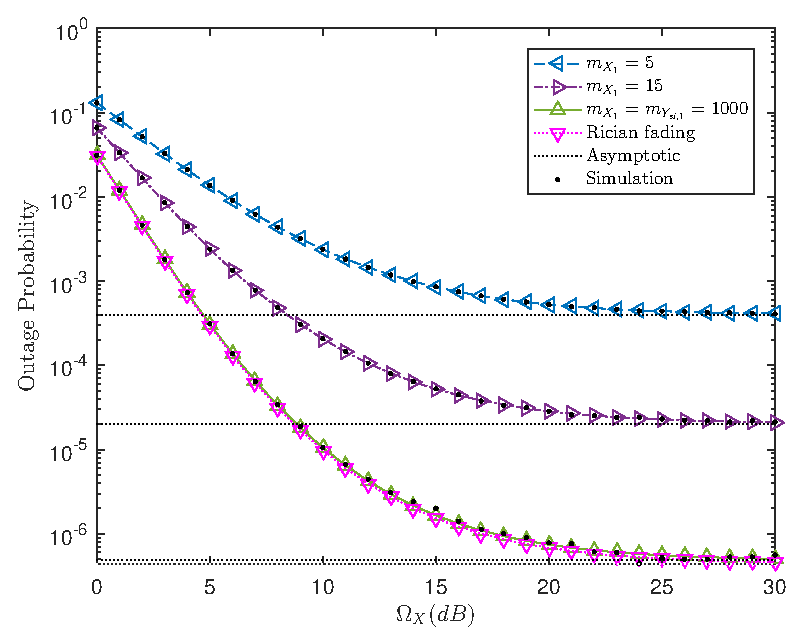
\includegraphics [width=0.45\columnwidth]{chap5_fig/gs_outage.eps}
\label{fig:HBD_UCS_Rician_Shadowed_gs_outage}}
\hfil
\subfloat[Impact of shadowing at GS for $\Omega_X = 5dB$ and $0.5 \leq m_{X_1}, m_{Y_{si,1}} \leq 15$.]{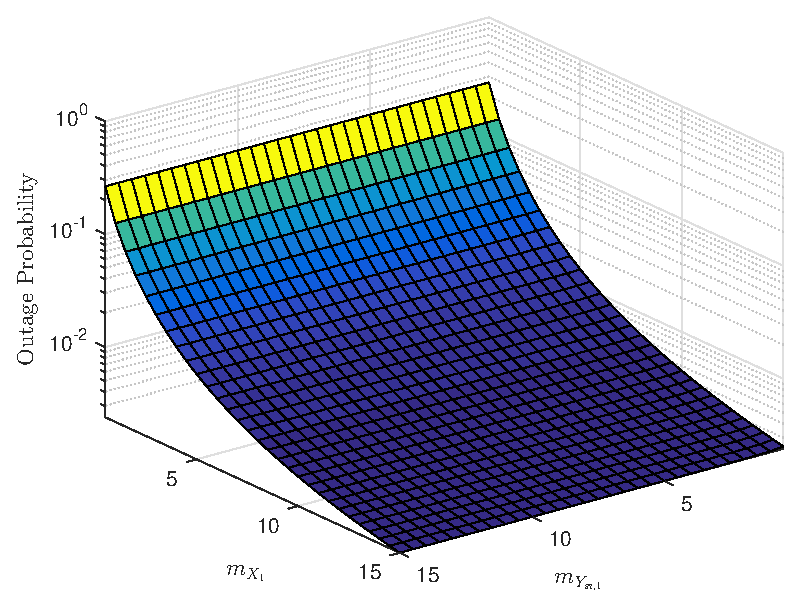
\includegraphics [width=0.45\columnwidth]{chap5_fig/gs_outage_surf.eps}
\label{fig:HBD_UCS_Rician_Shadowed_gs_outage_surf}}
\caption{Outage probability at GS for $\alpha_{g,g}=1$, $\epsilon=0.01$, $\gamma_{\phi}^2=-130$dBm, and $K_{X_1}=K_{Y_{si,1}}=15$.}
\end{figure*}

\begin{figure}[t]
\centering
\vspace{0.2cm}
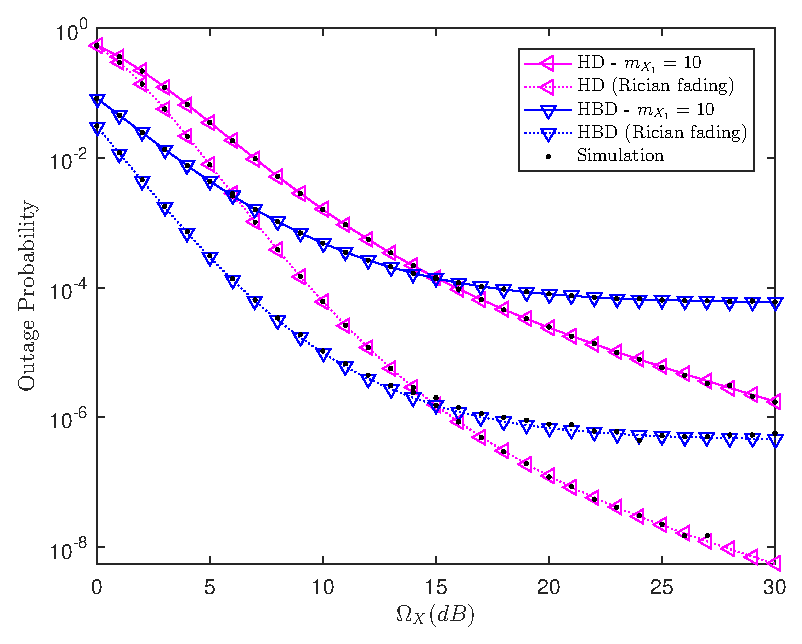
\includegraphics [width=0.45\columnwidth]{chap5_fig/gs_outage_HBD_vs_HD.eps} 
\caption{Outage probability at GS (HBD vs HD) for $\alpha_{g,g}=1$, $\epsilon=0.01$, $\gamma_{\phi}^2=-130$dBm, $K_{X_1}=K_{Y_{si,1}}=15$, $m_{Y_{si,1}}=10$.}
\label{fig:HBD_UCS_Rician_Shadowed_gs_outage_HBD_vs_HD}
\end{figure}

\begin{table}[t]
\centering 
\caption{Error margin of the outage probability at GS.}
\label{table:HBD_UCS_Rician_Shadowed_marg_gs}
\begin{tabular}{lccc}
\hline
																	& $\Omega_X = 5$ dB			& $\Omega_X = 15$ dB		& $\Omega_X = 30$ dB 		\\  \hline \hline
$m_{X_1}$ = 5 										& $4.68\times 10^{-5}$ 	& $2.74\times 10^{-5}$ 	& $1.14\times 10^{-5}$ 	\\
$m_{X_1}$ = 15 										& $1.34\times 10^{-6}$	& $8.59\times 10^{-6}$	& $8.51\times 10^{-6}$ 	\\
$m_{X_1}$ = $m_{Y_{si,1}}$ = 1000 & $1.98\times 10^{-6}$ 	&	-											& -											\\
Rician fading											& $1.25\times 10^{-5}$	& -											& -									 		\\
\hline
\end{tabular}
\end{table}

%%%%%%%%%%%%%%%%%%%%%%%%%%%%%%%%%%%%%%%%%%%%%%%%%%%%%%%%%%%%%%%%%%%%%%%%%%%%%%%%%%
% Impact of shadowing on the SI link is negligible on the outage probability at GS
% Large amounts of passive SI suppression results in less amounts of SI being mitigated at the active SI mitigation stage and vice-versa.
%%%%%%%%%%%%%%%%%%%%%%%%%%%%%%%%%%%%%%%%%%%%%%%%%%%%%%%%%%%%%%%%%%%%%%%%%%%%%%%%%%

\begin{observation}
\emph{\emph{Shadowing on the SI link has negligible impact on outage probability at the GS.}
}\end{observation}

The HBD outage probability at GS $\big(Pr\big(\mathcal{O}_{gs}^{HBD}\big)\big)$, given in (\ref{HBD_UCS_Rician_Shadowed_P_out_GS_HBD}), is shown in Fig. \ref{fig:HBD_UCS_Rician_Shadowed_gs_outage} for $m_{X_1} \in \{5, 15, 1000\}$. For the case of Rician fading channels, $Pr\big(\mathcal{O}_{gs}^{HBD}\big)$ is plotted using (\ref{HBD_UCS_Rician_Shadowed_P_out_GS_HBD_rician}) which matches with that using (\ref{HBD_UCS_Rician_Shadowed_P_out_GS_HBD}) for $m_{X_1}=m_{Y_{si,1}}=1000$. Likewise, $Pr\big(\mathcal{O}_{gs}^{HBD}\big)$ is plotted using (\ref{HBD_UCS_Rician_Shadowed_P_out_gs_HD_Rician}) for the case of Rician fading channels. The error margins of the outage probability at GS are shown in Table \ref{table:HBD_UCS_Rician_Shadowed_marg_gs}.

From Fig. \ref{fig:HBD_UCS_Rician_Shadowed_gs_outage}, it can be seen that the outage probability drops more steeply as $m_{X_1}$ increases due to less shadowing on the desired link $(h_{1,g})$ than the SI link $(h_{si})$. In Fig. \ref{fig:HBD_UCS_Rician_Shadowed_gs_outage_surf}, it is observed that shadowing on the SI link ($m_{Y_{si,1}}$) has negligible impact on the outage probability, especially when $m_{Y_{si,1}}$ is large. From Corollary \ref{HBD_UCS_Rician_Shadowed_frac_moments_corollary}, it is shown that the fractional moment of a Rician shadowed RV is independent of $m$ as $m \to \infty$. Therefore, the outage probability at the GS is independent of $m_{Y_{si,1}}$ as $m_{Y_{si,1}} \to \infty$. The trend in Fig. \ref{fig:HBD_UCS_Rician_Shadowed_gs_outage_surf} shows that having higher amounts of passive SI mitigation, i.e., smaller $m_{Y_{si,1}}$, will not further reduce outage probability at the FD-enabled GS. As SI is first mitigated at the passive SI suppression stage, residual SI is further mitigated at the active SI mitigation stage. Thus, large amounts of passive SI suppression results in less amounts of SI being mitigated at the active SI mitigation stage and vice-versa. A similar trend has also been seen in \cite[Fig. 9]{sahai2013impact}, where higher amounts of passive SI mitigation did not result in higher SI cancellation.

%%%%%%%%%%%%%%%%%%%%%%%%%%%%%%%%%%%%%%%%%%%%%%%%%%%%%%%%%%%%%%%%%%%%%%%%%%%%%%%%%%
% FD-enabled GS is more reliable than HD-GS (with or without shadowing).
%%%%%%%%%%%%%%%%%%%%%%%%%%%%%%%%%%%%%%%%%%%%%%%%%%%%%%%%%%%%%%%%%%%%%%%%%%%%%%%%%%

\begin{observation}
\emph{\emph{The FD-enabled GS is more reliable than the HD-GS at low SNR regimes, even in the presence of shadowing.}
}\end{observation}

In Fig. \ref{fig:HBD_UCS_Rician_Shadowed_gs_outage_HBD_vs_HD}, the HBD outage probability $\big(Pr\big(\mathcal{O}_{gs}^{HBD}\big)\big)$ and HD outage probability $\big(Pr\big(\mathcal{O}_{gs}^{HD}\big)\big)$ at GS are plotted, with the latter obtained from (\ref{HBD_UCS_Rician_Shadowed_P_out_gs_HD}). It can be seen in Fig. \ref{fig:HBD_UCS_Rician_Shadowed_gs_outage_HBD_vs_HD} that even in the presence of shadowing, the FD-enabled GS achieves lower outage probability at low SNR regimes than the HD-enabled GS. The FD-enabled GS also achieves better reliability in a shadowing environment than the HD-GS operating in a non-shadowing environment at low SNR regimes.    


% show plot for outage probability vs m_{X1} for Kx1 = {5,10,15}
\begin{figure} []
\centering
\vspace{0.2cm}
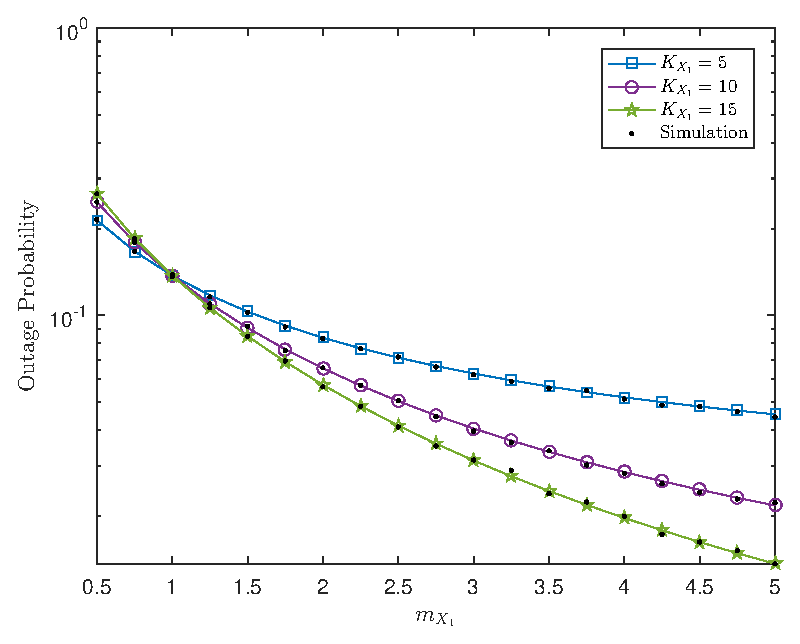
\includegraphics [width=0.45\columnwidth]{chap5_fig/gs_outage_mx1_vs_mysi1.eps} 
%\vspace{-0.5cm}
\caption{Impact of shadowing and Rician $K$ factors on outage probability at GS for $\Omega_X = 5$dB, $\alpha_{g,g}=1$, $\epsilon=0.01$, $\gamma_{\phi}^2=-130$dBm, $K_{Y_{si,1}}=10$, $m_{Y_{si,1}}=2$.}
%\vspace{-0.2cm}
\label{fig:HBD_UCS_Rician_Shadowed_gs_outage_mx1_vs_mysi1}
\end{figure}

%%%%%%%%%%%%%%%%%%%%%%%%%%%%%%%%%%%%%%%%%%%%%%%%%%%%%%%%%%%%%%%%%%%%%%%%%%%%%%%%%%
% when severe shadowing is experienced with strong LOS component, reliability is diminished even when SI mitigation measures are implemented.
%%%%%%%%%%%%%%%%%%%%%%%%%%%%%%%%%%%%%%%%%%%%%%%%%%%%%%%%%%%%%%%%%%%%%%%%%%%%%%%%%%

\begin{observation}
\emph{\emph{When severe shadowing is experienced with strong LOS component at the FD-enabled GS, reliability is diminished even when SI mitigation measures are implemented.}
}\end{observation}

In Fig \ref{fig:HBD_UCS_Rician_Shadowed_gs_outage_mx1_vs_mysi1}, the impact of shadowing and Rician $K$ factors on $Pr\big(\mathcal{O}_{gs}^{HBD}\big)$, from (\ref{HBD_UCS_Rician_Shadowed_P_out_GS_HBD}), is analyzed. Interestingly, it can be seen that $Pr\big(\mathcal{O}_{gs}^{HBD}\big)$ is high when the Rician $K$ factor is high and $m_{x_{1}} < 1$. Similar trends in \cite[Fig. 9]{kumar2017outage} have also been observed. A large Rician $K$ factor implies that the average received power of the scattered component is low. When $m$ is small, e.g, $m_{x_1} < 1$, severe shadowing on the LOS component is experienced. Under such circumstances, a large Rician $K$ factor causes overall average received power to be lower than when Rician $K$ factor is small. Also, from Corollaries \ref{HBD_UCS_Rician_Shadowed_rician_fading_alpha_corollary} and \ref{HBD_UCS_Rician_Shadowed_frac_moments_corollary}, the Rician $K$ factor has a positive influence on the outage probability when $m$ is large. Therefore, the opposite is also true, i.e., a small $m$ causes the Rician $K$ factor to negatively impact the outage probability. Thus, the reliability of the FD-enabled GS diminishes more as the Rician $K$ factor increases while the LOS component of the desired link $(h_{1,g})$ is obstructed, e.g., by buildings, despite the implementation of SI mitigation measures. To overcome the effect of shadowing on the desired link, relaying strategies can be considered.


\subsection{Impact of inter-UAV interference and Shadowing at UAV-2}
 
% show plot for JD outage probability vs omega_X for m_{xgs} = {5, 15} and alpha_{1.2} = {0.5, 0.7}. Include no shadowing plot (m = 1000)
% show plot for II outage probability vs omega_X for m_{xgs} = {5, 15} and alpha_{1.2} = {0.5, 0.7}. Include no shadowing plot (m = 1000)
\begin{figure*}[t]
\centering
\subfloat[Impact of shadowing on the II detector]{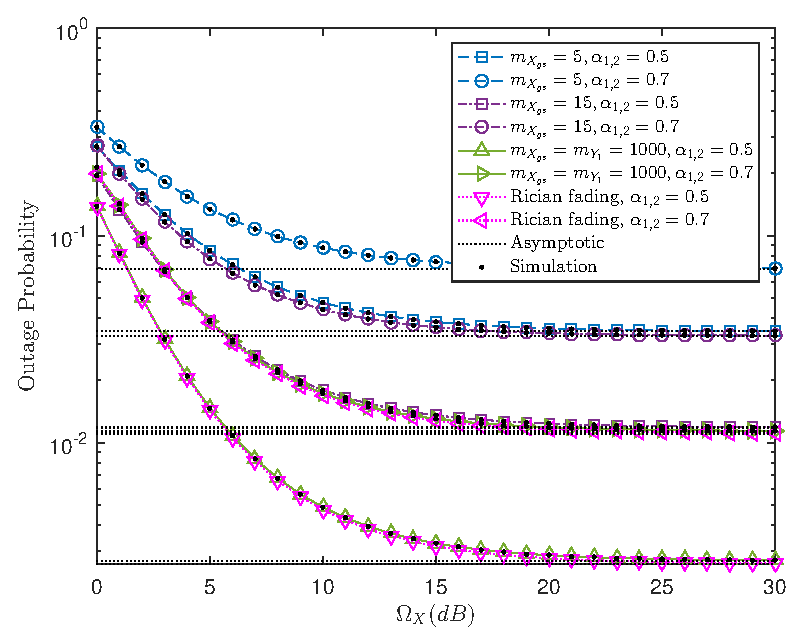
\includegraphics [width=0.45\columnwidth]{chap5_fig/uav2_II_outage.eps}
\label{fig:HBD_UCS_Rician_Shadowed_uav2_II_outage}}
\hfil
\subfloat[Impact of shadowing on the joint detector]{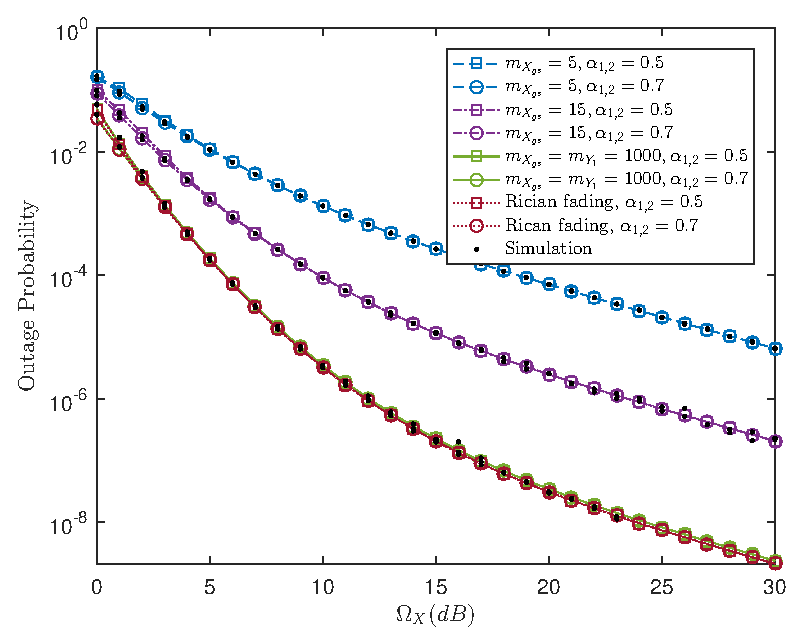
\includegraphics [width=0.45\columnwidth]{chap5_fig/uav2_JD_outage.eps} 
\label{fig:HBD_UCS_Rician_Shadowed_uav2_JD_outage}}
\caption{Outage probability at UAV-2 for $\alpha_{g,2}=1$, $K_{X_{gs}}=K_{Y_1}=15$, $m_{Y_1}=10$.}
\label{fig:HBD_UCS_Rician_Shadowed_uav2_outage}
\end{figure*}

\begin{table}[t]
\centering
\caption{Error margin of the outage probability at the ii and joint detectors for $\alpha_{1,2}=0.5$.}
\label{table:HBD_UCS_Rician_Shadowed_marg_II_JD} \scalebox{0.7}{
\begin{tabular}{lccc}
\hline
																						& $\Omega_X = 5$ dB			& $\Omega_X = 15$ dB		& $\Omega_X = 30$ dB 		\\  \hline \hline
$m_{X_{gs}}$ = 5 (II)												& $2.3\times 10^{-5}$ 	& $7.45\times 10^{-6}$ 	& $5.35\times 10^{-5}$ 	\\
$m_{X_{gs}}$ = 15 (II) 											& $3.6\times 10^{-6}$		& $3.34\times 10^{-5}$	& $2.6\times 10^{-5}$ 	\\
$m_{X_{gs}}$ = $m_{Y_{1}}$ = 1000 (II) 			& $6.91\times 10^{-5}$ 	&	$9.67\times 10^{-6}$	& $8.4\times 10^{-6}$	\\
Rician fading (II) 													& $3.8\times 10^{-4}$		& $1.47\times 10^{-4}$	& $9.46\times 10^{-5}$ 		\\
$m_{X_{X_{gs}}}$ = 5 (JD)										& $3.03\times 10^{-4}$ 	& $2.79\times 10^{-5}$	& - 										\\
$m_{X_{X_{gs}}}$ = 15 (JD)									& $5.34\times 10^{-5}$	& $8.1\times 10^{-7}$		& -											\\
$m_{X_{X_{gs}}}$ = $m_{Y_{1}}$ = 1000 (JD) 	& $1.17\times 10^{-6}$ 	&	-											& - 										\\
Rician fading (JD)													& $5.23\times 10^{-6}$	& -											& - 										\\
\hline
\end{tabular}}
\end{table}

%\begin{table}[]
%\centering
%\caption{\textcolor{black}{Error margin for outage probability at the joint detector for $\alpha_{1,2}=0.5$.}}
%\label{table:marg_JD}
%\begin{tabular}{cccc}
%\hline
																			%& $\Omega_X = 5$ dB			& $\Omega_X = 15$ dB		& $\Omega_X = 30$ dB		\\  \hline \hline
%$m_{X_{X_{gs}}}$ = 5 									& $3.03\times 10^{-4}$ 	& $2.79\times 10^{-5}$	& - 										\\
%$m_{X_{X_{gs}}}$ = 15 								& $5.34\times 10^{-5}$	& $8.1\times 10^{-7}$		& -											\\
%$m_{X_{X_{gs}}}$ = $m_{Y_{1}}$ = 1000 & $1.17\times 10^{-6}$ 	&	-											& - 										\\
%Rician fading 												& $5.23\times 10^{-6}$	& -											& - 										\\
%\hline
%\end{tabular}
%\end{table}

%%%%%%%%%%%%%%%%%%%%%%%%%%%%%%%%%%%%%%%%%%%%%%%%%%%%%%%%%%%%%%%%%%%%%%%%%%%%%%%%%%
% Shadowing on the desired link has the equivalent effect of higher inter-UAV interference on the received signal at the II detector.
% Shadowing on the desired link and inter-UAV interference causes the II detector to have diminished reliability.
% The reliability of the II-based HBD-UCS is diminished when deployed in urban environments with large numbers of UAVs.
%%%%%%%%%%%%%%%%%%%%%%%%%%%%%%%%%%%%%%%%%%%%%%%%%%%%%%%%%%%%%%%%%%%%%%%%%%%%%%%%%%

\begin{observation}
\emph{\emph{Severe shadowing on the desired link has the equivalent impact of higher inter-UAV interference at the II detector, which results in diminished reliability.}
}\end{observation}

The HBD outage probability for the II detector $\big(Pr\big(\mathcal{O}_{2}^{HBD(II)}\big)\big)$ at UAV-2, computed from (\ref{HBD_UCS_Rician_Shadowed_P_out_uav2_II_HBD}), is plotted in Fig. \ref{fig:HBD_UCS_Rician_Shadowed_uav2_II_outage} for $m_{X_{gs}} \in \{5, 15, 1000\}$ and $\alpha_{1,2} \in \{0.5, 0.7\}$. Also, $Pr\big(\mathcal{O}_{2}^{HBD(II)}\big)$ is plotted in Fig. \ref{fig:HBD_UCS_Rician_Shadowed_uav2_II_outage} for the II detector over Rician fading channels using (\ref{HBD_UCS_Rician_Shadowed_P_out_uav2_II_HBD_rician}), where it is seen to be matching with (\ref{HBD_UCS_Rician_Shadowed_P_out_uav2_II_HBD}) for $m_{X_{gs}}=m_{Y_1}=1000$ and $\alpha_{1,2} \in \{0.5, 0.7\}$. For HD-UCS, $Pr\big(\mathcal{O}_{2}^{HD}\big)$ is plotted using (\ref{HBD_UCS_Rician_Shadowed_P_out_uav2_HD_Rician}). The error margins of the outage probability at UAV-2 are shown in Table \ref{table:HBD_UCS_Rician_Shadowed_marg_II_JD}.

In Fig. \ref{fig:HBD_UCS_Rician_Shadowed_uav2_II_outage}, similar observations seen in Fig. \ref{fig:HBD_UCS_Rician_Shadowed_gs_outage} are noted. Specifically, a lower $Pr\big(\mathcal{O}_{2}^{HBD(II)}\big)$ is attained when the desired link ($h_{g,2}$) experiences less severe shadowing than the interfering link ($h_{1,2}$), i.e., $m_{X_{gs}} > m_{Y_1}$. Also, for $m_{X_{gs}}=5$ and $\alpha_{1,2}=0.5$, $Pr\big(\mathcal{O}_{2}^{HBD(II)}\big)$ is similar to that obtained for $m_{X_{gs}}=15$ and $\alpha_{1,2}=0.7$. Similar observations are also made for the case of $m_{X_{gs}}=15$ and $\alpha_{1,2}=0.5$, and $m_{X_{gs}}=1000$ and $\alpha_{1,2}=0.7$. Therefore, severe shadowing on the desired link has the equivalent effect of higher inter-UAV interference levels on the received signal at the II detector. From Fig. \ref{fig:HBD_UCS_Rician_Shadowed_uav2_II_outage}, it is apparent that both shadowing on the desired link and inter-UAV interference causes the II detector to have diminished reliability. Thus, deploying the II detector-based HBD-UCS for multi-UAV networks in urban environments results in diminished reliability. Such a limitation inadvertently places constraints on the overall QoS requirements for the multi-UAV network.   

%%%%%%%%%%%%%%%%%%%%%%%%%%%%%%%%%%%%%%%%%%%%%%%%%%%%%%%%%%%%%%%%%%%%%%%%%%%%%%%%%%
% combined effect of shadowing and inter-UAV interference affects the outage probability decay rate at low SNR regimes.
% multi-UAV IoT platforms with joint detector-based HBD-UCS can achieve higher reliability, especially in urban environments.
%%%%%%%%%%%%%%%%%%%%%%%%%%%%%%%%%%%%%%%%%%%%%%%%%%%%%%%%%%%%%%%%%%%%%%%%%%%%%%%%%%

\begin{observation}
\emph{\emph{Shadowing and inter-UAV interference reduces the outage probability decay rate of the joint detector at low SNR regimes.}
}\end{observation}

The HBD outage probability for the joint detector $\big(Pr\big(\mathcal{O}_{2}^{HBD(JD)}\big)\big)$ at UAV-2, computed from (\ref{HBD_UCS_Rician_Shadowed_P_out_uav2_JD_HBD}), is plotted in Fig. \ref{fig:HBD_UCS_Rician_Shadowed_uav2_JD_outage} for $m_{X_{gs}} \in \{5, 15\}$ and $\alpha_{1,2} \in \{0.5, 0.7\}$. For reference, $Pr\big(\mathcal{O}_{2}^{HBD(JD)}\big)$ is plotted in Fig. \ref{fig:HBD_UCS_Rician_Shadowed_uav2_JD_outage} over Rician fading channels using (\ref{HBD_UCS_Rician_Shadowed_P_out_uav2_JD_HBD_rician}) to reflect the outage probability at the joint detector in the absence of shadowing. 

From Fig. \ref{fig:HBD_UCS_Rician_Shadowed_uav2_JD_outage}, the effect of shadowing on the joint detector is more pronounced than inter-UAV interference, especially at moderate and high SNR regimes. Since the joint detector works well in the presence of strong interference \cite{zahavi2017cooperation,zhou2015mac,shubhi2017joint,blomer2009transmission}, it is not interference-limited at high SNR regimes. Instead, the combined effect of shadowing and inter-UAV interference reduces the outage probability decay rate at low SNR regimes. When $m_{X_{gs}} = 15$ and $\alpha_{1,2} \in \{0.5, 0.7\}$, $Pr\big(\mathcal{O}_{2}^{HBD(JD)}\big)$ decays more steeply, as compared to setting $m_{X_{gs}} = 5$ and $\alpha_{1,2} \in \{0.5, 0.7\}$. Thus, the joint detector exhibits higher reliability when $\alpha_{1,2} \to \infty$ and $m_{X_{gs}} > m_{Y_1}$. In contrast to the II detector, multi-UAV networks with joint detector-based HBD-UCS can achieve higher reliability, especially in urban environments.

%%%%%%%%%%%%%%%%%%%%%%%%%%%%%%%%%%%%%%%%%%%%%%%%%%%%%%%%%%%%%%%%%%%%%%%%%%%%%%%%%%
% The proposed HBD-UCS shows superior reliability over HD-UCS, with the joint detector clearly outperforming the II detector in terms of reliability.
%%%%%%%%%%%%%%%%%%%%%%%%%%%%%%%%%%%%%%%%%%%%%%%%%%%%%%%%%%%%%%%%%%%%%%%%%%%%%%%%%%

\begin{observation}
\emph{\emph{In the presence of inter-UAV interference and shadowing, the joint detector exhibits lower outage probability than the II detector and the HD-UCS at low SNR regimes.}
}\end{observation}

\begin{figure} [t]
\centering
\vspace{0.2cm}
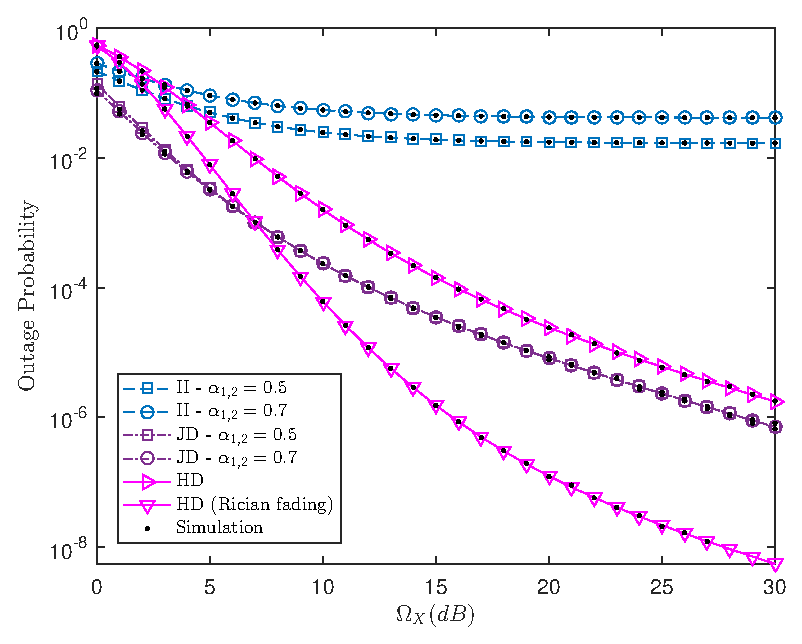
\includegraphics [width=0.45\columnwidth]{chap5_fig/uav2_II_vs_JD_outage.eps} 
%\vspace{-0.5cm}
\caption{Comparison between the II and joint detectors at UAV-2 for $\alpha_{g,2}=1$, $K_{X_{gs}}=K_{Y_1}=15$, $m_{X_{gs}}=m_{Y_1}=10$.}
%\vspace{-0.2cm}
\label{fig:HBD_UCS_Rician_Shadowed_uav2_II_vs_JD_outage}
\end{figure}

In Fig. \ref{fig:HBD_UCS_Rician_Shadowed_uav2_II_vs_JD_outage}, the HBD outage probability of the II detector $\big(Pr\big(\mathcal{O}_{2}^{HBD(II)}\big)\big)$ and the joint detector $\big(Pr\big(\mathcal{O}_{2}^{HBD(JD)}\big)\big)$ are plotted. In addition, the HD-UCS outage probability at UAV-2 $\big(Pr\big(\mathcal{O}_{2}^{HD}\big)\big)$ is also plotted using (\ref{HBD_UCS_Rician_Shadowed_P_out_uav2_HD}). As reference, $Pr\big(\mathcal{O}_{2}^{HD}\big)$ in the absence of shadowing is provided using (\ref{HBD_UCS_Rician_Shadowed_rician_cdf}) by substituting $\Omega = \Omega_X\alpha_{g,2}$, $K=K_{X_{gs}}$, and $\gamma=\gamma_{th,2}^{HD}$.

\begin{figure} [t]
\centering
\vspace{0.2cm}
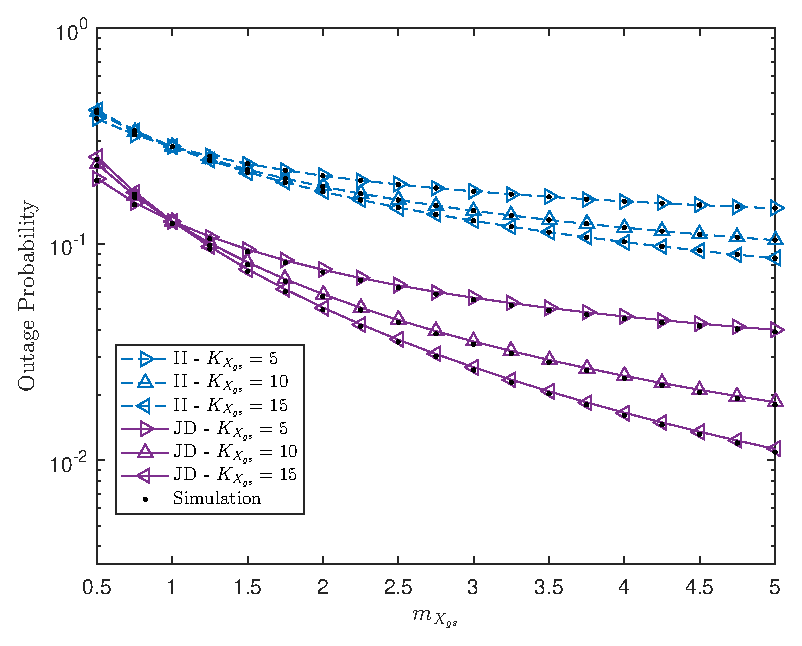
\includegraphics [width=0.45\columnwidth]{chap5_fig/uav2_outage_mxgs_vs_my1.eps} 
%\vspace{-0.5cm}
\caption{Impact of shadowing and Rician $K$ factors on outage probability at UAV-2 for $\Omega_X = 5$dB, $\alpha_{g,2}=1$, $\alpha_{1,2}=0.5$, $K_{Y_1}=10$, $m_{Y_1}=10$.}
%\vspace{-0.2cm}
\label{fig:HBD_UCS_Rician_Shadowed_uav2_outage_mxgs_vs_my1}
\end{figure}

From Fig. \ref{fig:HBD_UCS_Rician_Shadowed_uav2_II_vs_JD_outage}, outage probability trends observed for the II detector in \cite[Fig. 4]{tan2018ricianShad} are also seen in Fig. \ref{fig:HBD_UCS_Rician_Shadowed_uav2_II_vs_JD_outage}. Specifically, it is seen in Fig. \ref{fig:HBD_UCS_Rician_Shadowed_uav2_II_vs_JD_outage} that the II detector attained lower outage probability than the HD-UCS at low SNR regimes. The same is also observed when the HD-UCS is not experiencing the effects of shadowing, i.e., HD-UCS over Rician fading channels. However, at high SNR regimes, the II detector is observed to be interference-limited due to the error floor observed in Fig. \ref{fig:HBD_UCS_Rician_Shadowed_uav2_II_vs_JD_outage}.

For the joint detector, the attained outage probability is \textcolor{black}{lower than that of} HD-UCS when shadowing is considered. When shadowing is not experienced at the HD-UCS, the joint detector achieves lower outage probability for $\Omega_X < 7$dB. In addition, the superiority of the joint detector over the II detector is highlighted. Therefore, the HBD-UCS shows superior reliability over HD-UCS. The joint detector clearly outperforms the II detector in terms of reliability. Thus, the former is more suitable for multi-UAV networks with high QoS requirements.

%%%%%%%%%%%%%%%%%%%%%%%%%%%%%%%%%%%%%%%%%%%%%%%%%%%%%%%%%%%%%%%%%%%%%%%%%%%%%%%%%%
% The joint detector shows higher reliability than the II detector in severe shadowing environments.
%%%%%%%%%%%%%%%%%%%%%%%%%%%%%%%%%%%%%%%%%%%%%%%%%%%%%%%%%%%%%%%%%%%%%%%%%%%%%%%%%%

\begin{observation}
\emph{\emph{Severe shadowing with strong LOS component has less effect on the joint detector than on the II detector.}
}\end{observation}

In Fig. \ref{fig:HBD_UCS_Rician_Shadowed_uav2_outage_mxgs_vs_my1}, the same observations made in Fig. \ref{fig:HBD_UCS_Rician_Shadowed_gs_outage_mx1_vs_mysi1} are noted. Thus, severe shadowing on the desired link $(h_{g,2})$ with large Rician $K$ factor diminishes the reliability of the II and joint detectors. However, the effect is less extensive for the joint detector than the II detector since outage probability of the former is lower than the latter. As such, the superiority of the joint detector over the II detector is highlighted in severe shadowing environments, e.g., urban environments. 

%%%%%%%%%%%%%%%%%%%%%%%%%%%%%%%%%%%%%%%%%%%%%%%%%%%%%%%%%%%%%%%%%%%%%%%%%%%%%%%%%%%%%%%%%%%%%%%%%%%%%%%%%%%%%%%%%%%%%%%%%%%%%%%%%%%%%%%%%
% Section 6: Conclusion
\section{Chapter Summary} \label{HBD_UCS_Rician_Shadowed_sec_conclusion}
An HBD-UCS, consisting of HD UAVs and FD GSs, is investigated as an alternative to address spectrum scarcity in UAV communications. To effectively model the underlying communication channels, Rician shadowed fading is assumed on all links to account for shadowing introduced in urban environments. To this end, an innovative mathematical framework is presented to obtain alternative closed-form representations related to both the Rician shadowed fading and the Rician fading models. Closed-form outage probability expressions for the II and the joint detectors are then obtained from the derived expressions. An extensive outage probability analysis of the HBD-UCS was conducted under various inter-UAV interference and shadowing scenarios over Rician shadowed fading channels. At the GS, the impact of shadowing on the desired link and the SI link was demonstrated. Specifically, at the GS, shadowing on the desired link impacts the outage probability considerably. On the other hand, shadowing on the SI link has negligible impact on GS outage probability. Additionally, it is also demonstrated the GS operates with lower outage probability in FD mode than in HD mode. At UAV-2, it was shown that the joint detector attains lower outage probability than the II detector and the HD-UCS. The robustness of the joint detector under severe shadowing on the desired link was also demonstrated. Thus, the superior reliability and robustness of the joint detectors makes it an ideal candidate for multi-UAV networks operating in congested urban environments. 

It is also important to note that the analysis in this chapter, as well as the preceding chapters, focused on the specific case of two UAVs in the HBD-UCS. To this end, the performance of the HBD-UCS is analyzed in the next chapter for arbitrary number of UAVs deployed in an HBD multi-UAV network.



